\documentclass[10pt]{article}
\usepackage[margin=0.75in]{geometry}
\usepackage[T1]{fontenc}
\usepackage[utf8]{inputenc}
\usepackage{graphicx}
\usepackage{booktabs}
\usepackage{array}
\usepackage{longtable}
\usepackage{amsmath,amssymb}
\usepackage{caption}
\usepackage{hyperref}

\newcolumntype{L}[1]{>{\raggedright\arraybackslash}p{#1}}
\newcommand{\clip}{\operatorname{clip}_{[0,1]}}
\renewcommand{\thetable}{S\arabic{table}}
\renewcommand{\thefigure}{S\arabic{figure}}
\captionsetup[table]{name=Supplementary Table,labelsep=period}
\captionsetup[figure]{name=Supplementary Fig.,labelsep=period}
\setlength{\parindent}{15pt}
\setlength{\parskip}{0pt}

\title{Supplementary Information\\
A Physiology-Aligned State-Space Decomposition Framework for Camera-Derived Respiratory Motion}
\author{Young-Jae Cho and Dae-Yeol Kim}
\date{}

\begin{document}
\maketitle

\section*{Supplementary Methods}

\subsection*{Target-computable reliability law}
The reliability evidence used by PARH-OSSM is computed before access to the
target respiratory reference. Each candidate observation contributes
target-computable features describing rate agreement, preprocessing invariance,
event timing, bridge timing, rate/phase support, morphology support, ROI
observability, harmonic ambiguity, nuisance pressure, and abstention pressure.
Reference-derived or oracle columns are removed before materialization of the
evaluated runs.

All reliability features are mapped to $[0,1]$ by clipping. Let $G$ denote
group support, $M$ macro timing, $B$ bridge timing, $P$ rate/phase support,
$O_{\mathrm{roi}}$ ROI observability, $O_{\mathrm{prep}}$ preprocessing
invariance, $T$ timing reliability, $E$ event timing, $U$ nuisance pressure,
$H$ harmonic-risk score, $H_g$ harmonic-guard score, $R_m$ morphology
reliability, $M_s$ morphology support, $R$ generic reliability, and $A_b$
abstention pressure. The component-law implementation uses the fixed
combinations
\[
A=\clip(0.35G+0.25M+0.20B+0.20P),\qquad
O=\clip\{\sqrt{O_{\mathrm{roi}}O_{\mathrm{prep}}}\},
\]
\[
T^\ast=\clip\{T(1-0.55H)\},
\]
\[
w_{h1}=\clip\{T^\ast(0.55+0.25E+0.20A)(0.65+0.35O)(1-0.45U)\},
\]
\[
w_{h2}=\clip\{M_s(0.45+0.35H_g+0.20G)(0.65+0.35O)(1-0.30U)\},
\]
\[
w_b=\clip\{(0.45O_{\mathrm{prep}}+0.35O_{\mathrm{roi}}+0.20R)(1-0.35U)\},
\]
\[
N_m=\clip\{\max(R_m-T,0)\},
\]
\[
w_r=\clip\{(0.55M_s+0.25G+0.20N_m)(0.70+0.30O)(1-0.55U)\},
\]
and
\[
A_c=\clip\{\max(A_b,\ H(1-T),\ U(1-G),\ 0.75(1-O))\}.
\]
The oscillatory readout anchor and full-waveform readout weights are then
\[
w_{z_{\mathrm{osc}}}=\clip\{w_{h1}(1-0.50A_c)\},
\]
\[
w_{z_{\mathrm{full}}}=\clip\{(0.35w_{h1}+0.25w_{h2}+0.20w_b+0.20w_r)(1-0.35A_c)\}.
\]
These weights are responsibilities for state and readout roles, not a
ground-truth selector. They modulate observation trust and process-noise
allocation; respiratory labels are used only for evaluation and post hoc
oracle analyses.

\section*{Supplementary Tables}

\begin{longtable}{L{1.9cm}L{2.35cm}L{2.65cm}L{3.65cm}L{3.20cm}}
\caption{Dataset and evidence scope.}\\
\toprule
Dataset & Role & Label scope & Main use & Claim boundary \\
\midrule
\endfirsthead
\toprule
Dataset & Role & Label scope & Main use & Claim boundary \\
\midrule
\endhead
COHFACE & Primary real benchmark & Respiration waveform and derived rate & Rate, aligned waveform, strict waveform, and cycle diagnostics & Supports clean-regime real waveform/rate claims. \\
MAHNOB-HCI & Hard real benchmark & Respiration-belt waveform and derived rate & Rate, aligned waveform, strict waveform, and observability taxonomy & Supports hard-regime boundary analysis; low observability is reported explicitly. \\
V4V & External real rate-only evidence & Frame-aligned RR labels; no raw respiratory waveform & External rate-scope check & Does not support waveform morphology claims. \\
SCAMPS & Synthetic diagnostic control & Synthetic breathing signal and video arrays & Controlled mechanism and distribution diagnostics & Not mixed with real-data performance claims. \\
\bottomrule
\end{longtable}

This table defines the evidence boundary used throughout the manuscript. The
real-data claims come from COHFACE and MAHNOB-HCI, whereas V4V and SCAMPS are
retained only for rate-scope or diagnostic context. This separation prevents
external or synthetic controls from being mixed into the real waveform
benchmark.

\begin{longtable}{L{1.65cm}L{3.0cm}L{2.75cm}L{2.45cm}L{3.20cm}}
\caption{Fixed observation-class map.}\\
\toprule
Class & Construction & Primary information & Nuisance risk & PARH-OSSM role \\
\midrule
\endfirsthead
\toprule
Class & Construction & Primary information & Nuisance risk & PARH-OSSM role \\
\midrule
\endhead
OF & Raw vertical optical-flow surrogate & Oscillatory motion and local phase/frequency & Medium & Helper-heavy rate evidence. \\
OF bridge & OF-derived displacement-compatible bridge & Bridged oscillatory displacement & Medium & Rate-oriented constructed cue. \\
DoF & Thresholded frame-difference count & Thresholded motion energy & High & Auxiliary nuisance-limited cue. \\
DoF bridge & Signed DoF motion-centroid trajectory & Coarse signed motion trajectory & High & Hard-regime signed-motion probe. \\
P1D linear & Linear one-dimensional profile shift & Fundamental displacement & Medium & Conservative displacement cue. \\
P1D quadratic & Quadratic one-dimensional profile shift & Harmonic morphology and asymmetry & Low & Waveform-primary harmonic cue. \\
P1D cubic & Cubic one-dimensional profile shift & Harmonic morphology and asymmetry & Low & Waveform-primary harmonic cue. \\
P1D consensus & Weighted consensus of P1D routes & Consensus displacement morphology & Low & Agreement and morphology-support cue. \\
\bottomrule
\end{longtable}

This table is the nomenclature map for the fixed observation bank. The eight
classes are not interchangeable preprocessing variants: they expose different
motion cues, nuisance risks, and likely roles in the PARH-OSSM state/readout
pipeline. The table therefore supports the main-text claim that observability
must be analysed at the observation-class level.

\begin{longtable}{L{4.65cm}L{8.70cm}}
\caption{Supplementary data files included with the release package.}\\
\toprule
File & Purpose \\
\midrule
\endfirsthead
\toprule
File & Purpose \\
\midrule
\endhead
Strict waveform CSV & Strict zero-lag waveform metrics and span-normalized reconstruction diagnostics. \\
Cycle timing CSV & Cycle timing companion metrics for peak, trough, and peak-to-peak intervals. \\
Readout-alignment ablation CSV & COHFACE readout-alignment ablation supporting rate/waveform role separation. \\
Component-ablation evidence CSV & Component-level evidence and claim-boundary ledger. \\
Diagnostics CSV & Calibration diagnostics, including PARH NIS and Student-\(t\) weights. \\
Observation-class comparison CSV & Complete fixed-observation, OSSM-KF, and PARH-OSSM diagnostic comparison. \\
Paired statistical comparison CSV & Paired common-subset effect-size deltas used to interpret MAHNOB-HCI fairly. \\
\bottomrule
\end{longtable}

This table links the numerical claims to the released audit artifacts. It
distinguishes strict waveform metrics, observation-class comparisons, and
paired common-subset statistics so that readers can reproduce the main claims
without treating diagnostic-only files as hidden model-selection inputs.

\clearpage
\section*{Supplementary Figures}

\begin{figure}[htbp]
\centering
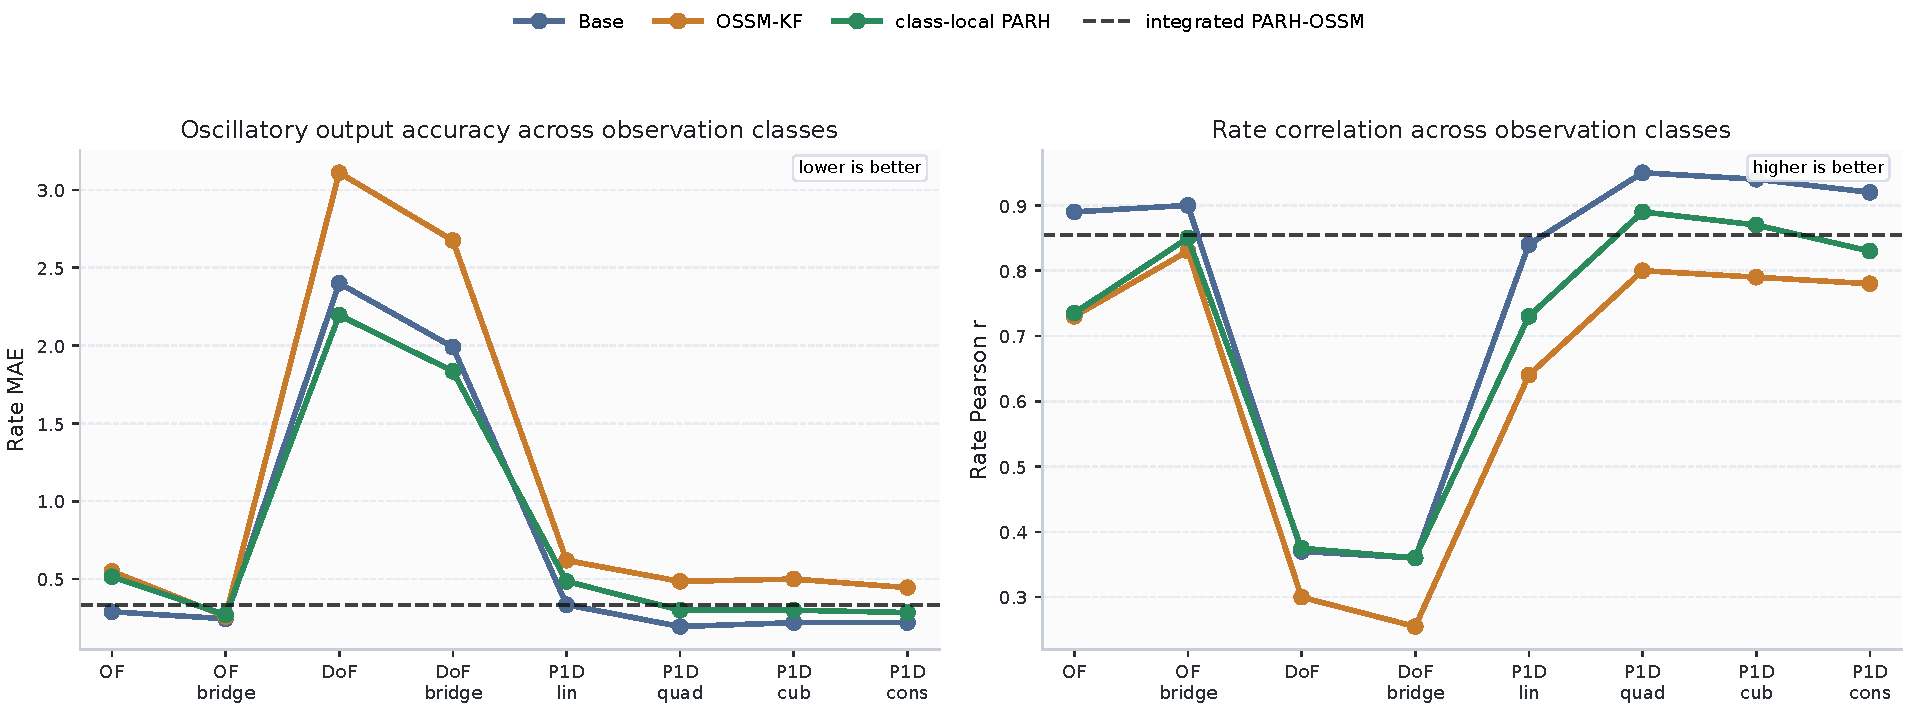
\includegraphics[width=\linewidth]{figures/F3_rate_observation_class_summary.pdf}
\caption{Complete eight-observation rate diagnostic plot. The figure compares direct observations, OSSM-KF, and observation-class-local PARH timing behavior across the fixed observation classes and is used only as diagnostic context, not as a target-specific best-source selector.}
\end{figure}

This figure expands the rate evidence beyond the three compact rows in the
main text. It shows whether fixed observations, OSSM-KF, and PARH-style readouts
fail for the same reason or for different observation-class reasons. Because it
is diagnostic, it explains the observed boundary but does not define a
target-specific best-source policy.

\begin{figure}[htbp]
\centering
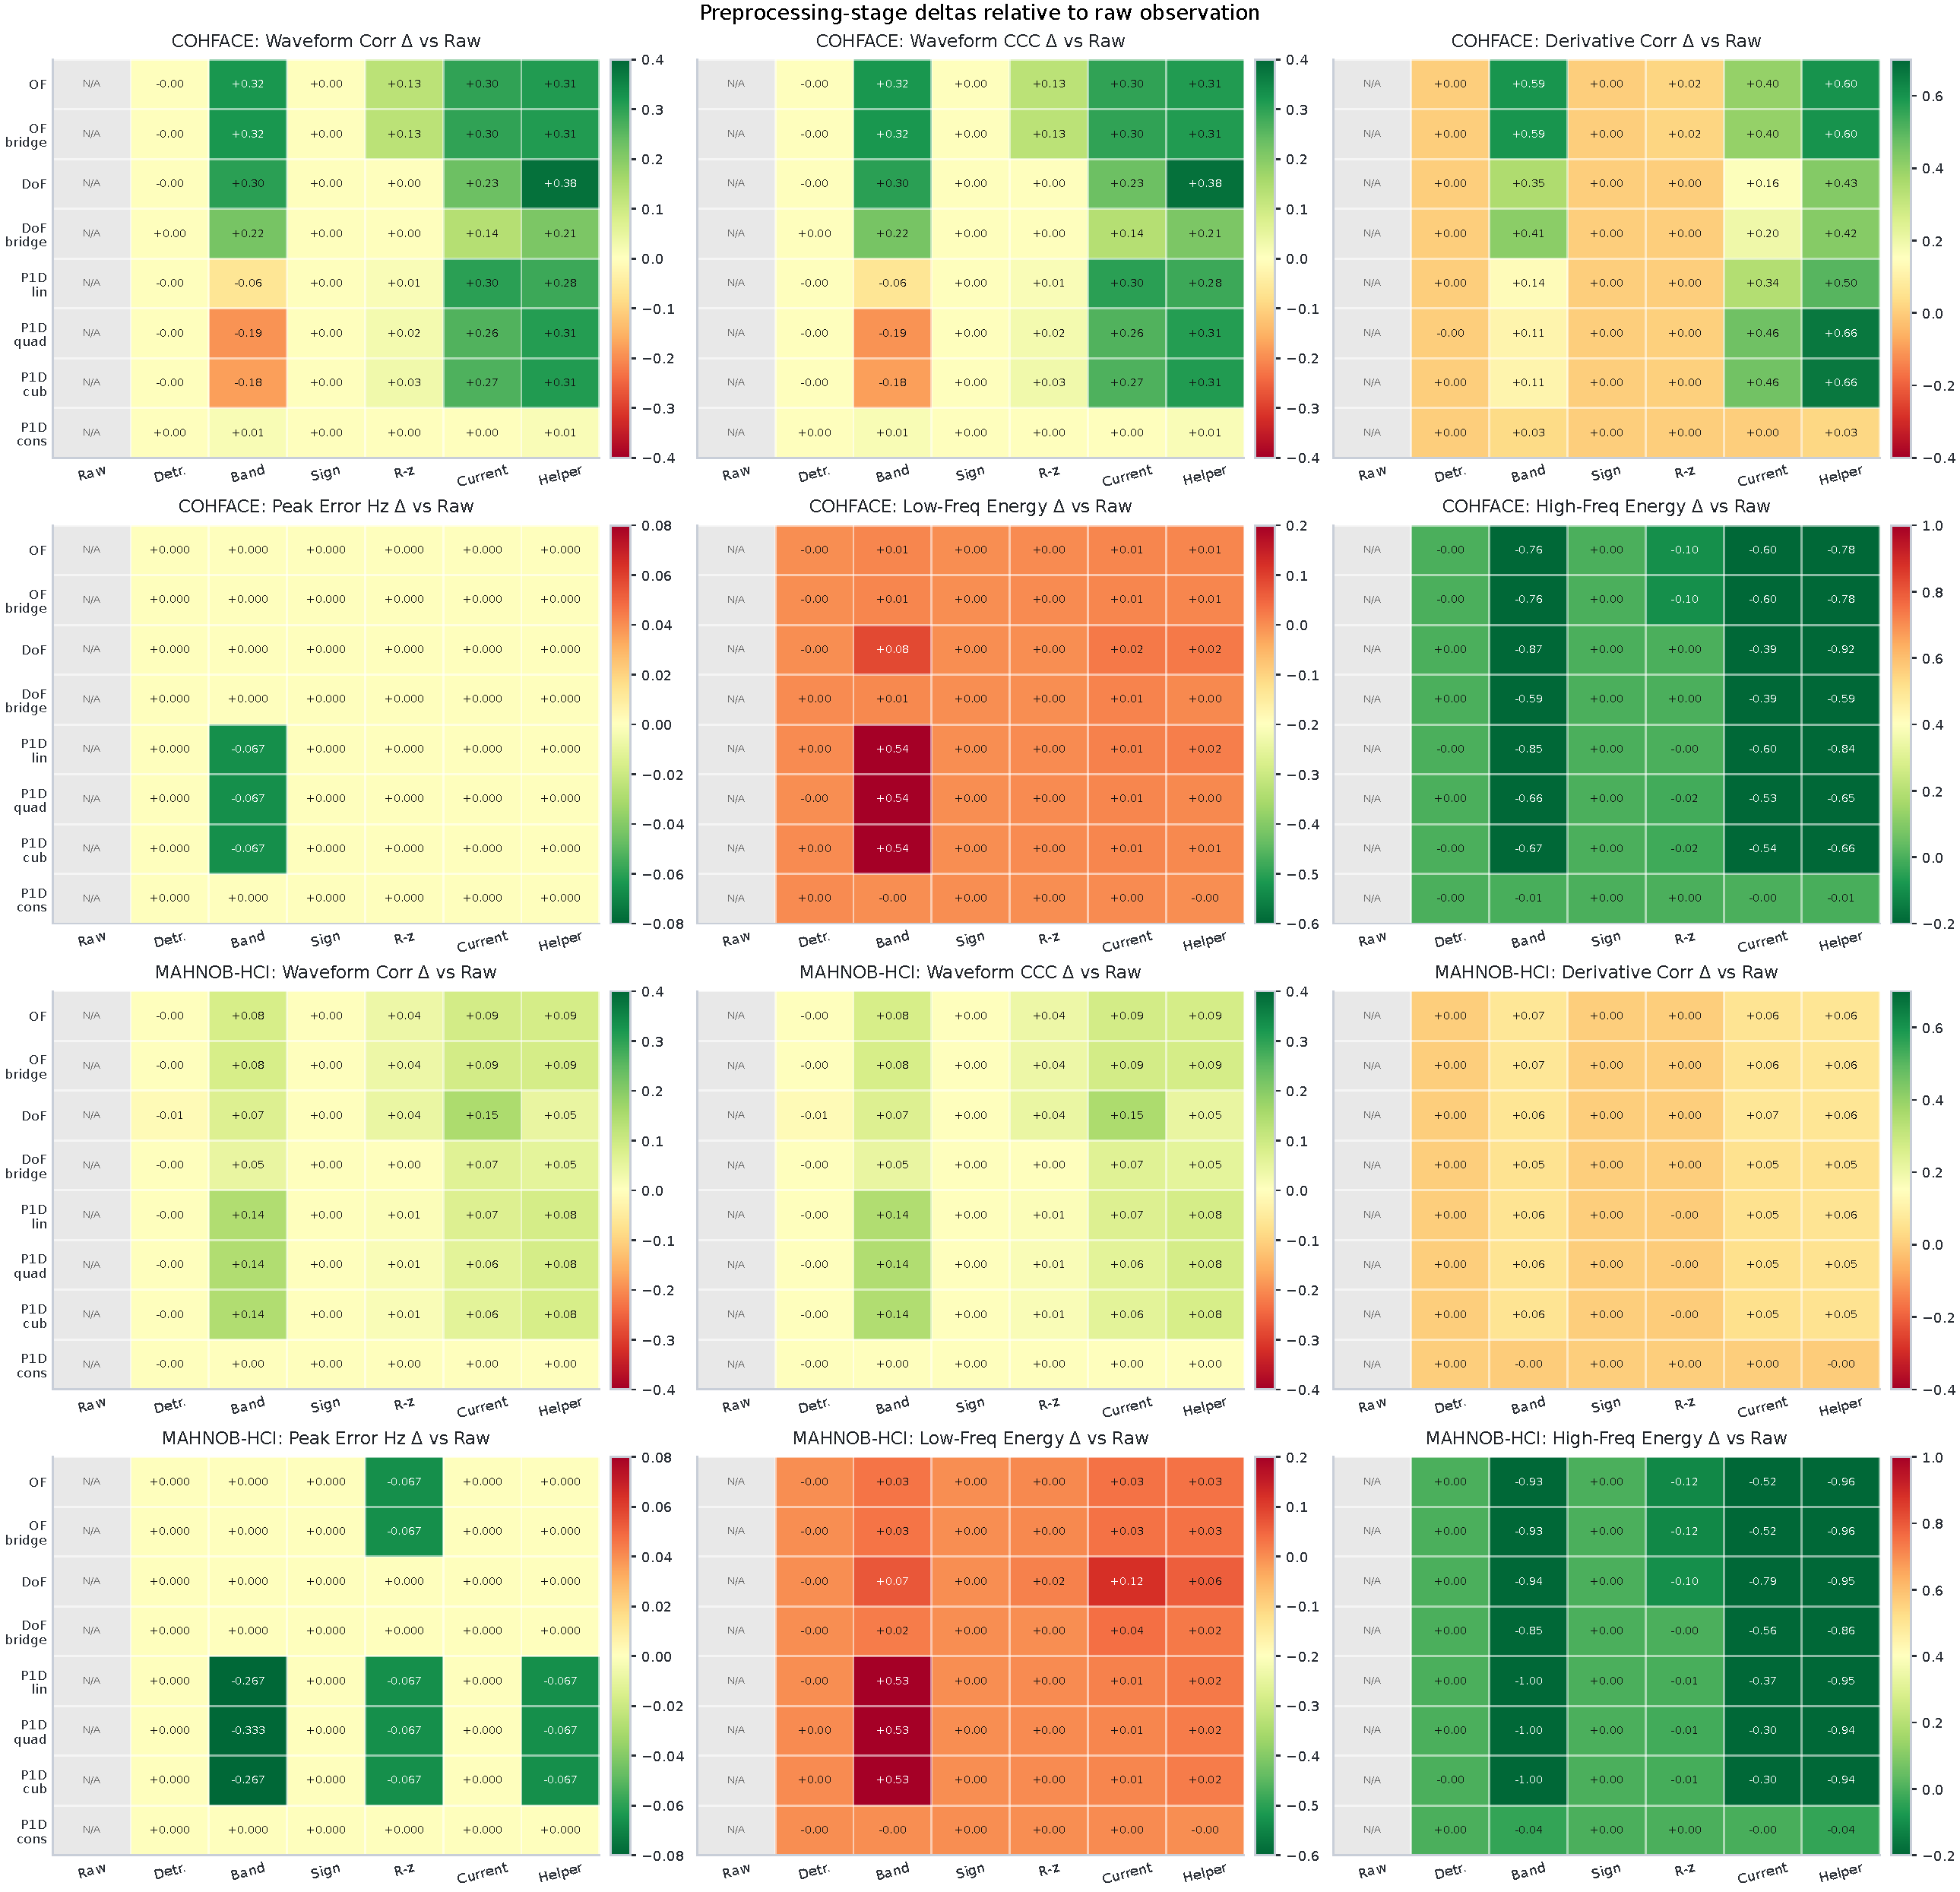
\includegraphics[width=\linewidth]{figures/S_F5_preproc_delta_heatmaps.pdf}
\caption{Preprocessing-stage delta heatmaps. The figure shows how raw, detrended, band-limited, sign-coded, robustly scaled, current-path, and helper views alter observation quality before state-space inference.}
\end{figure}

This figure localizes where observation quality changes before the latent state
model is applied. The preprocessing views should therefore be read as parallel
evidence transformations, not as a single ordered cascade. Their main purpose is
to show which cues survive simple transformations and which become
nuisance-dominated.

\begin{figure}[htbp]
\centering
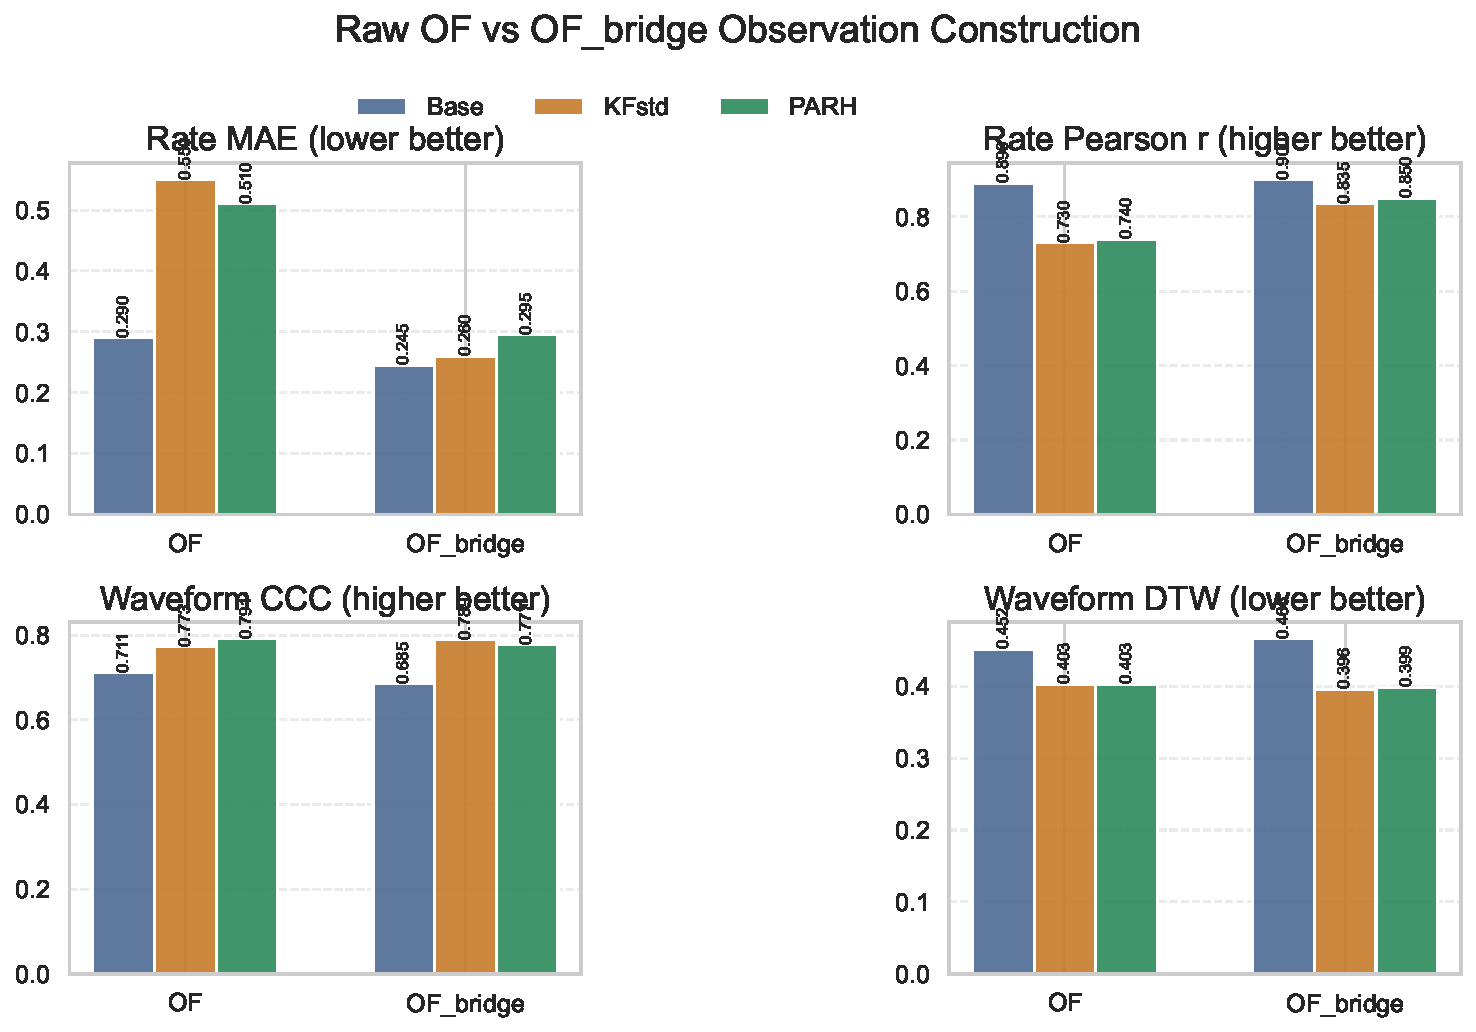
\includegraphics[width=0.86\linewidth]{figures/S_F6_of_construction_comparison.pdf}
\caption{Optical-flow construction comparison. The raw optical-flow route and the displacement-compatible bridge are shown as distinct observation constructions rather than interchangeable preprocessing variants.}
\end{figure}

This figure clarifies why OF and OF-bridge are kept as separate observation
routes. Raw optical flow and the bridged displacement-compatible cue can differ
in rate support, waveform topology, and failure mode, so collapsing them would
hide a construction-level source of evidence.

\begin{figure}[htbp]
\centering
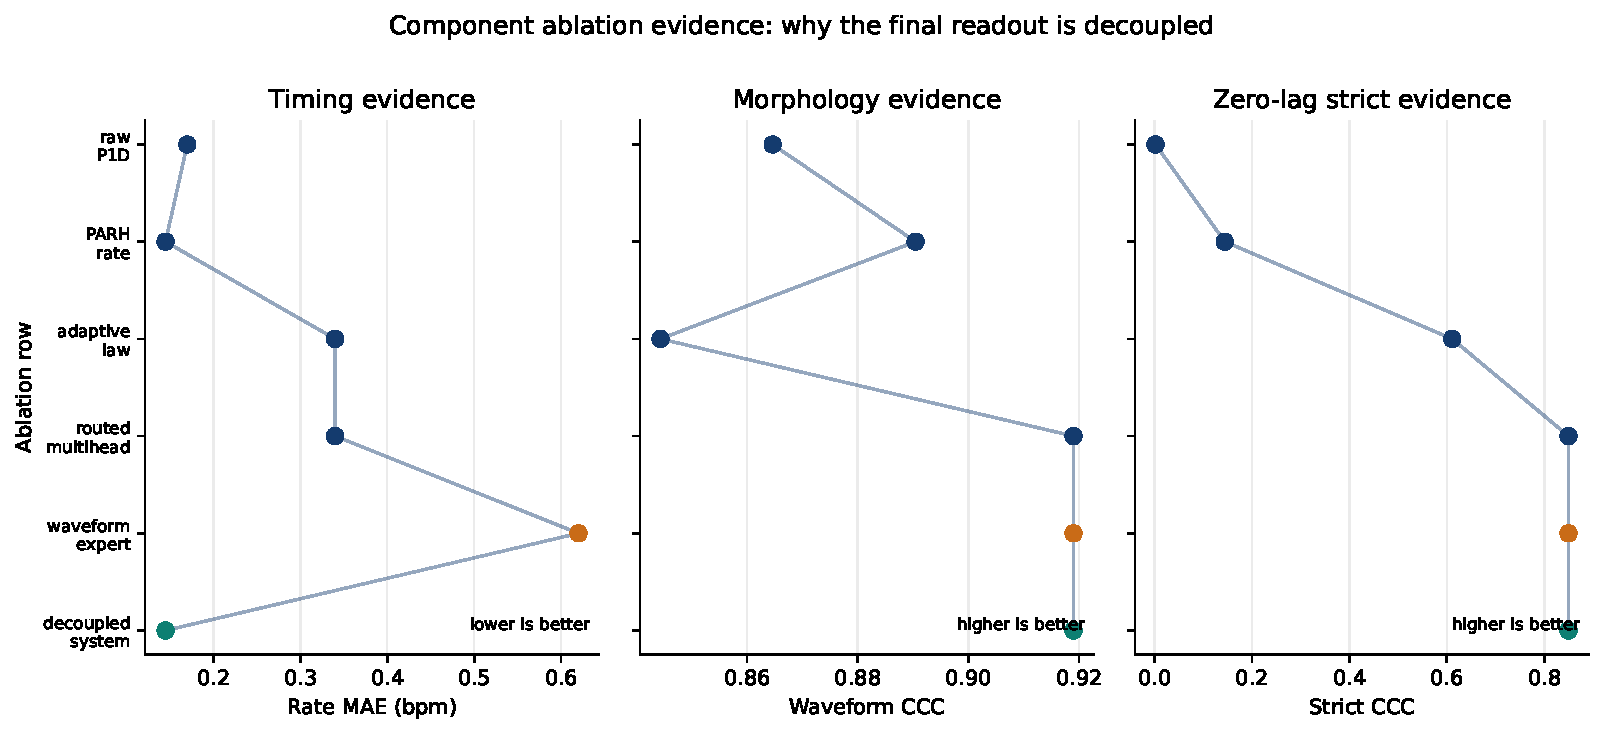
\includegraphics[width=0.86\linewidth]{figures/S_F_component_ablation_evidence.pdf}
\caption{Component-ablation evidence summary. The figure separates performance-bearing architecture evidence from diagnostic or construction-only components.}
\end{figure}

This figure defines which explored components are supported by numeric
performance evidence and which are retained only as diagnostics or construction
probes. It guards against overclaiming by making the difference between
promoted architecture and audit evidence explicit.

\begin{figure}[htbp]
\centering
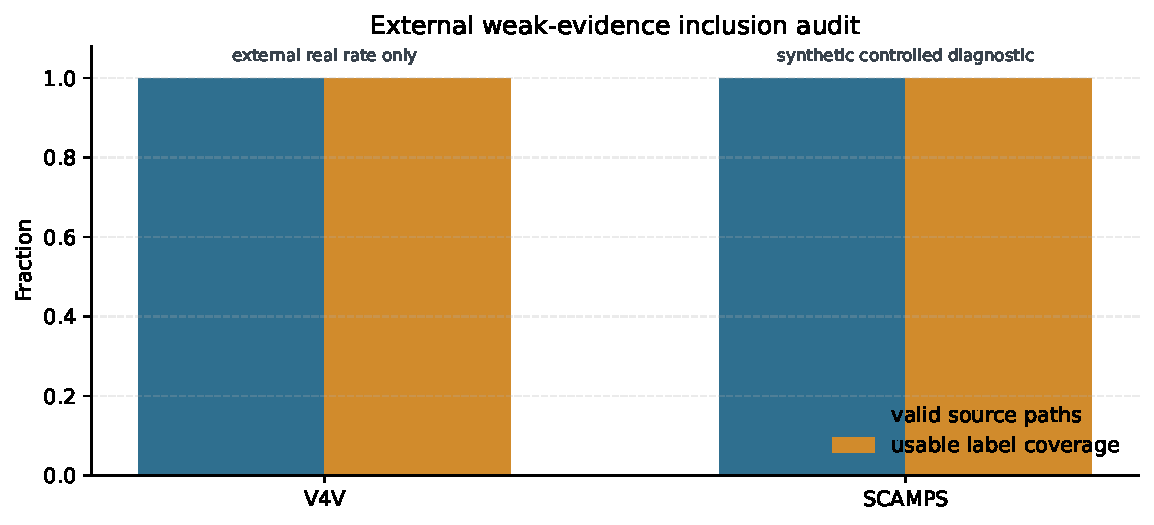
\includegraphics[width=0.80\linewidth]{figures/S_F_external_weak_evidence_summary.pdf}
\caption{External weak-evidence summary. V4V and SCAMPS document rate-label and synthetic-control scope but are not pooled into the real waveform benchmark metrics.}
\end{figure}

This figure explains the role of datasets that are informative but not part of
the main waveform benchmark. V4V contributes external rate-label context and
SCAMPS contributes synthetic diagnostic control, but neither supports the
real-video waveform morphology claims made from COHFACE and MAHNOB-HCI.

\begin{figure}[htbp]
\centering
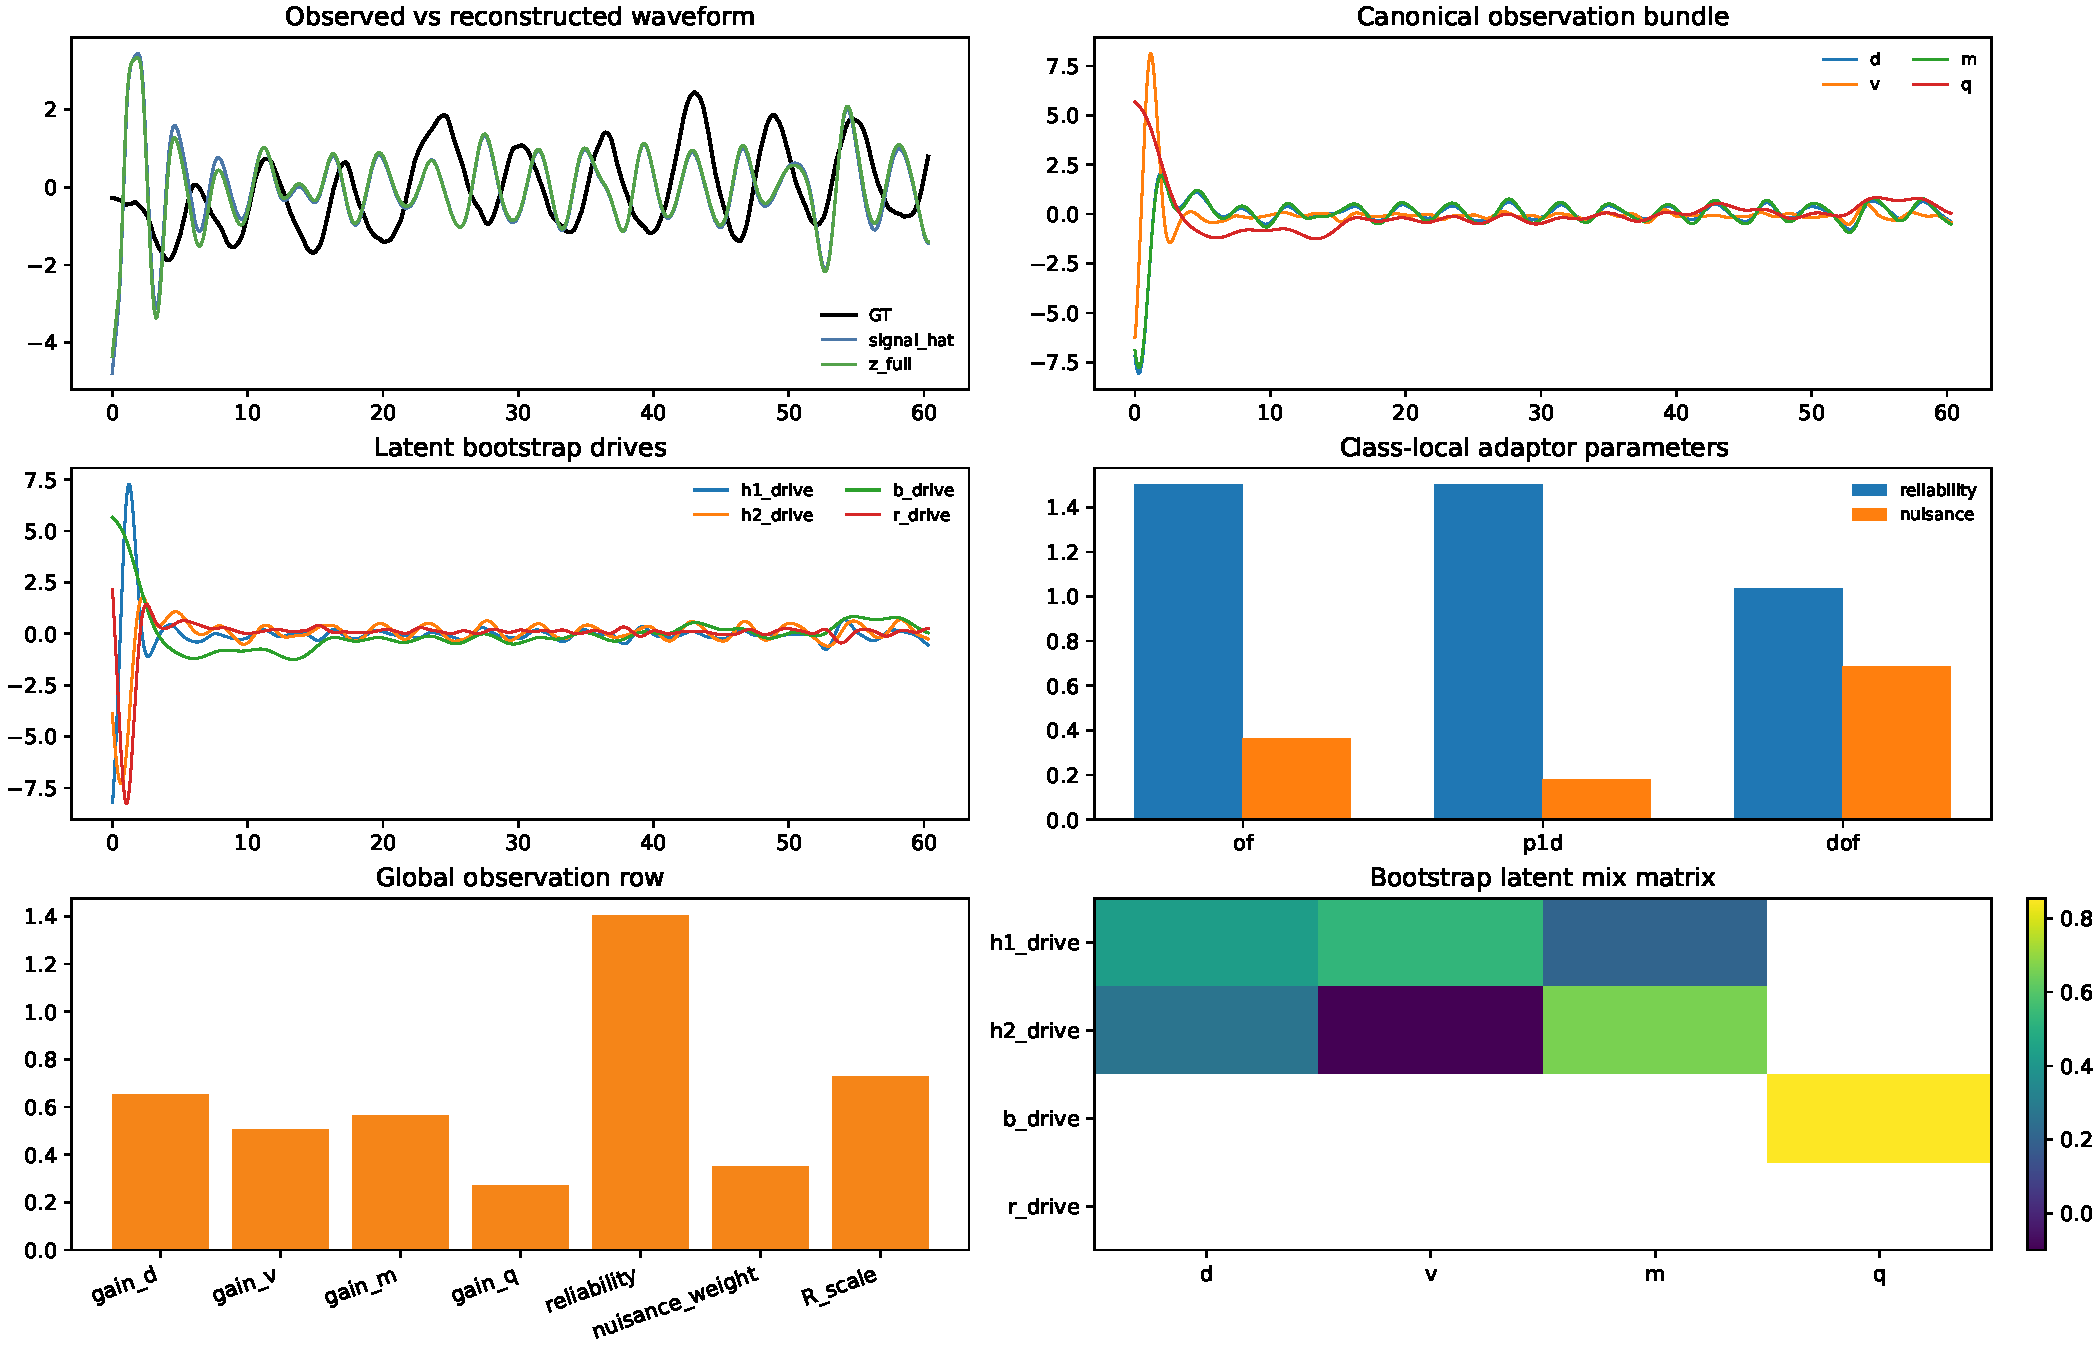
\includegraphics[width=0.90\linewidth]{figures/S_F9_state_bundle_diagnostics.pdf}
\caption{State-bundle and latent-bootstrap diagnostics. The figure visualizes the diagnostic observation summaries and latent state-drive traces retained to inspect the observation-to-state interface.}
\end{figure}

This figure exposes the interface between candidate evidence and latent state
roles. It helps readers check whether harmonic, baseline, and residual drives
are being activated by plausible observation summaries rather than by an
unreported oracle source.

\begin{figure}[htbp]
\centering
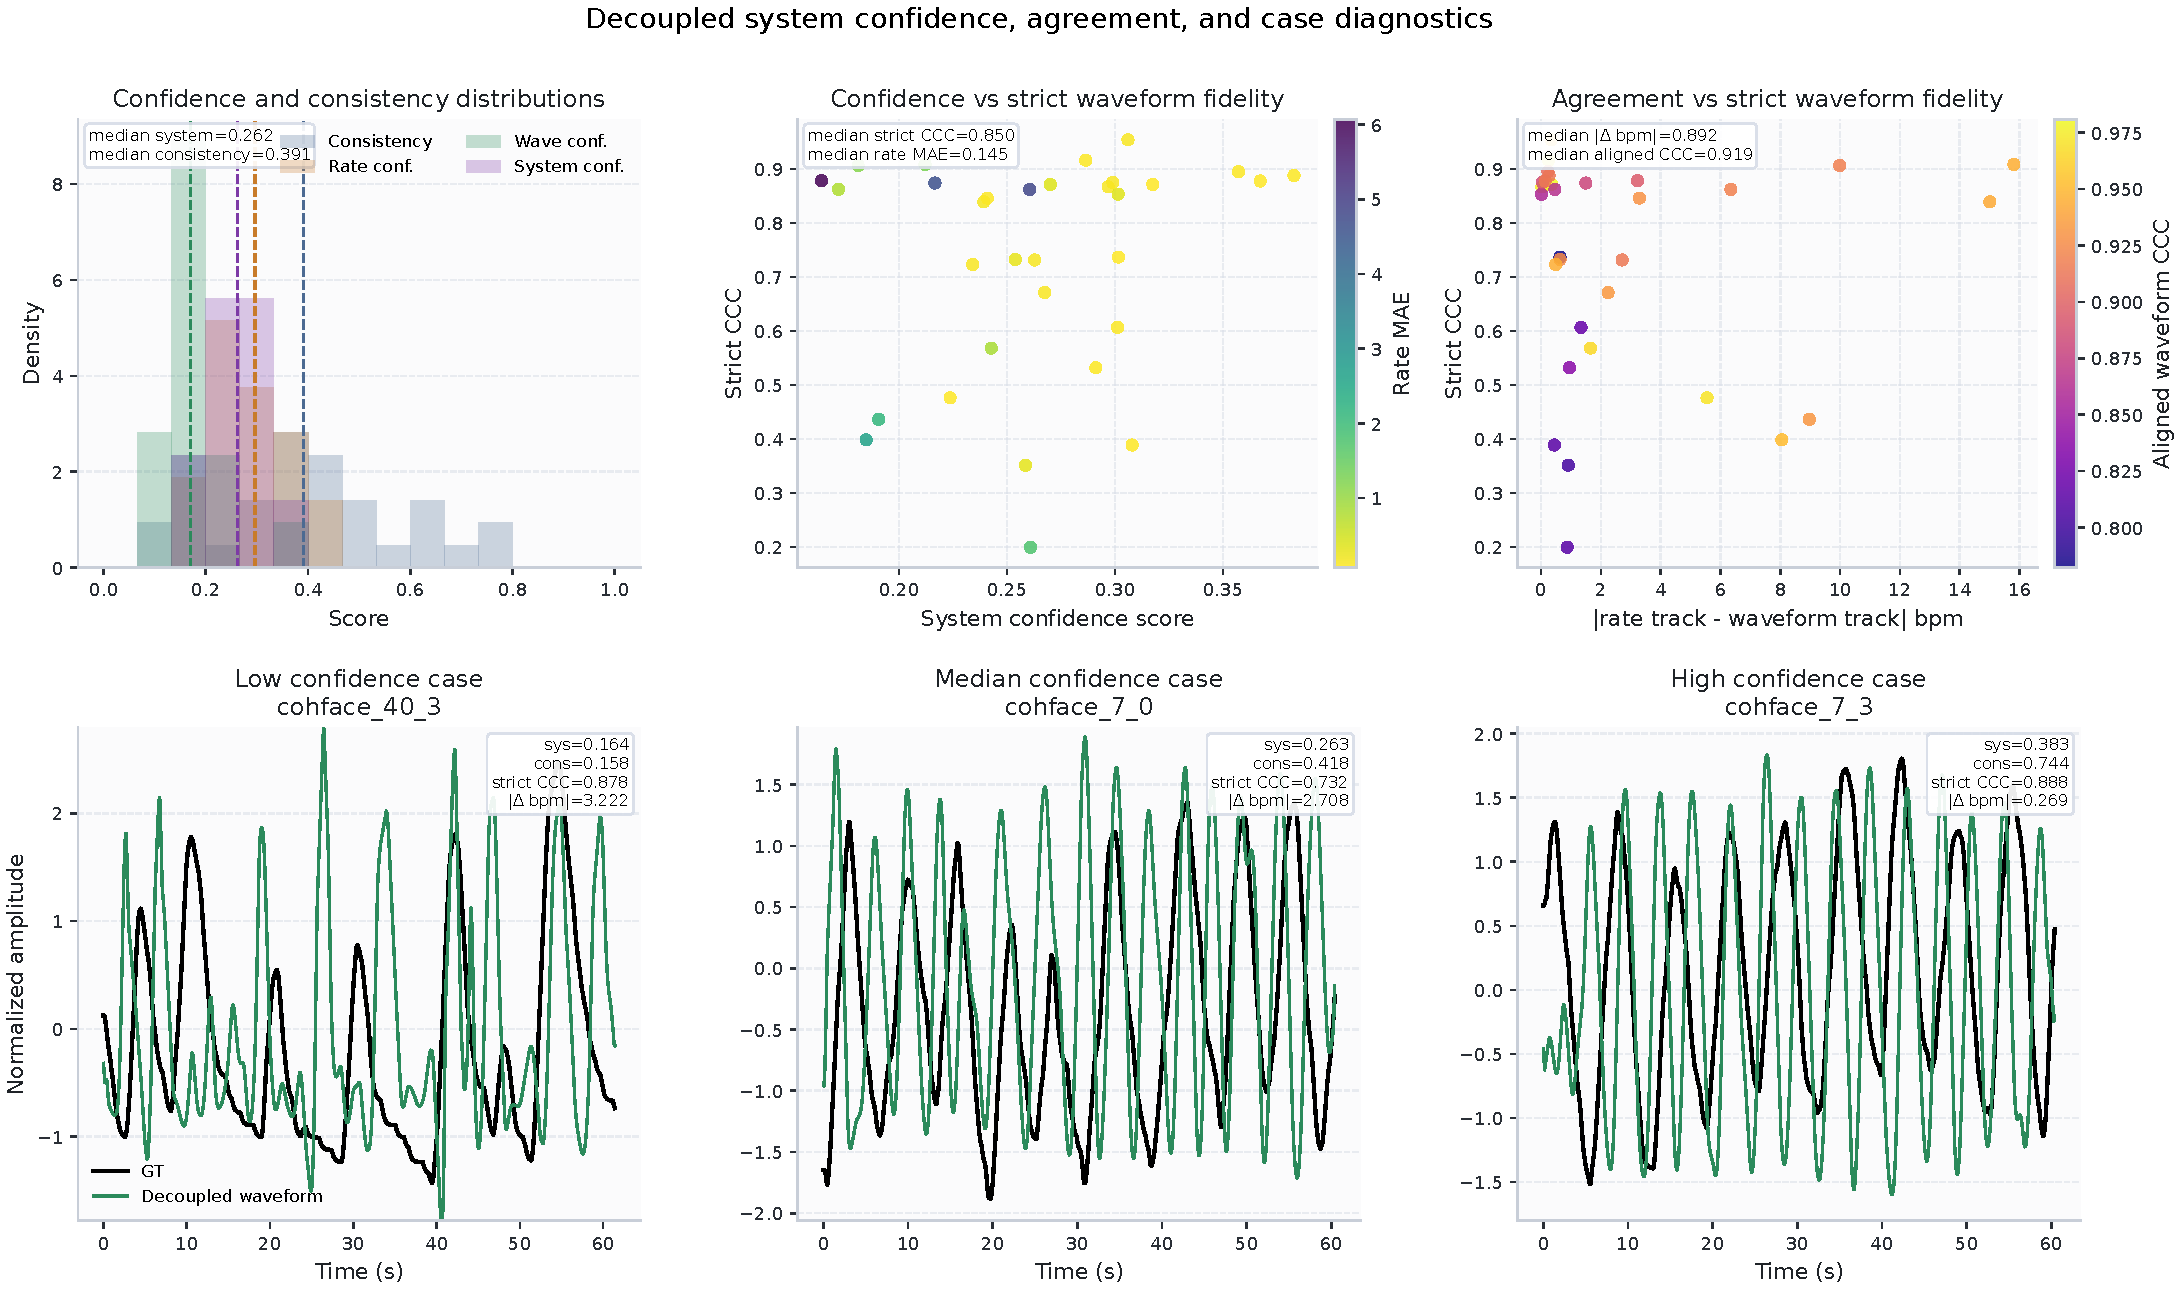
\includegraphics[width=0.90\linewidth]{figures/S_F10_decoupled_system_diagnostics.pdf}
\caption{Decoupled-system confidence and rate-waveform agreement diagnostics. The figure summarizes why oscillatory and full-waveform readouts are interpreted separately.}
\end{figure}

This figure supports the dual-readout interpretation in the main text. It shows
that confidence and agreement can differ between the oscillatory rate path and
the full waveform path, which is why $z_{\mathrm{osc}}$ and
$z_{\mathrm{full}}$ are not evaluated as the same target.

\begin{figure}[htbp]
\centering
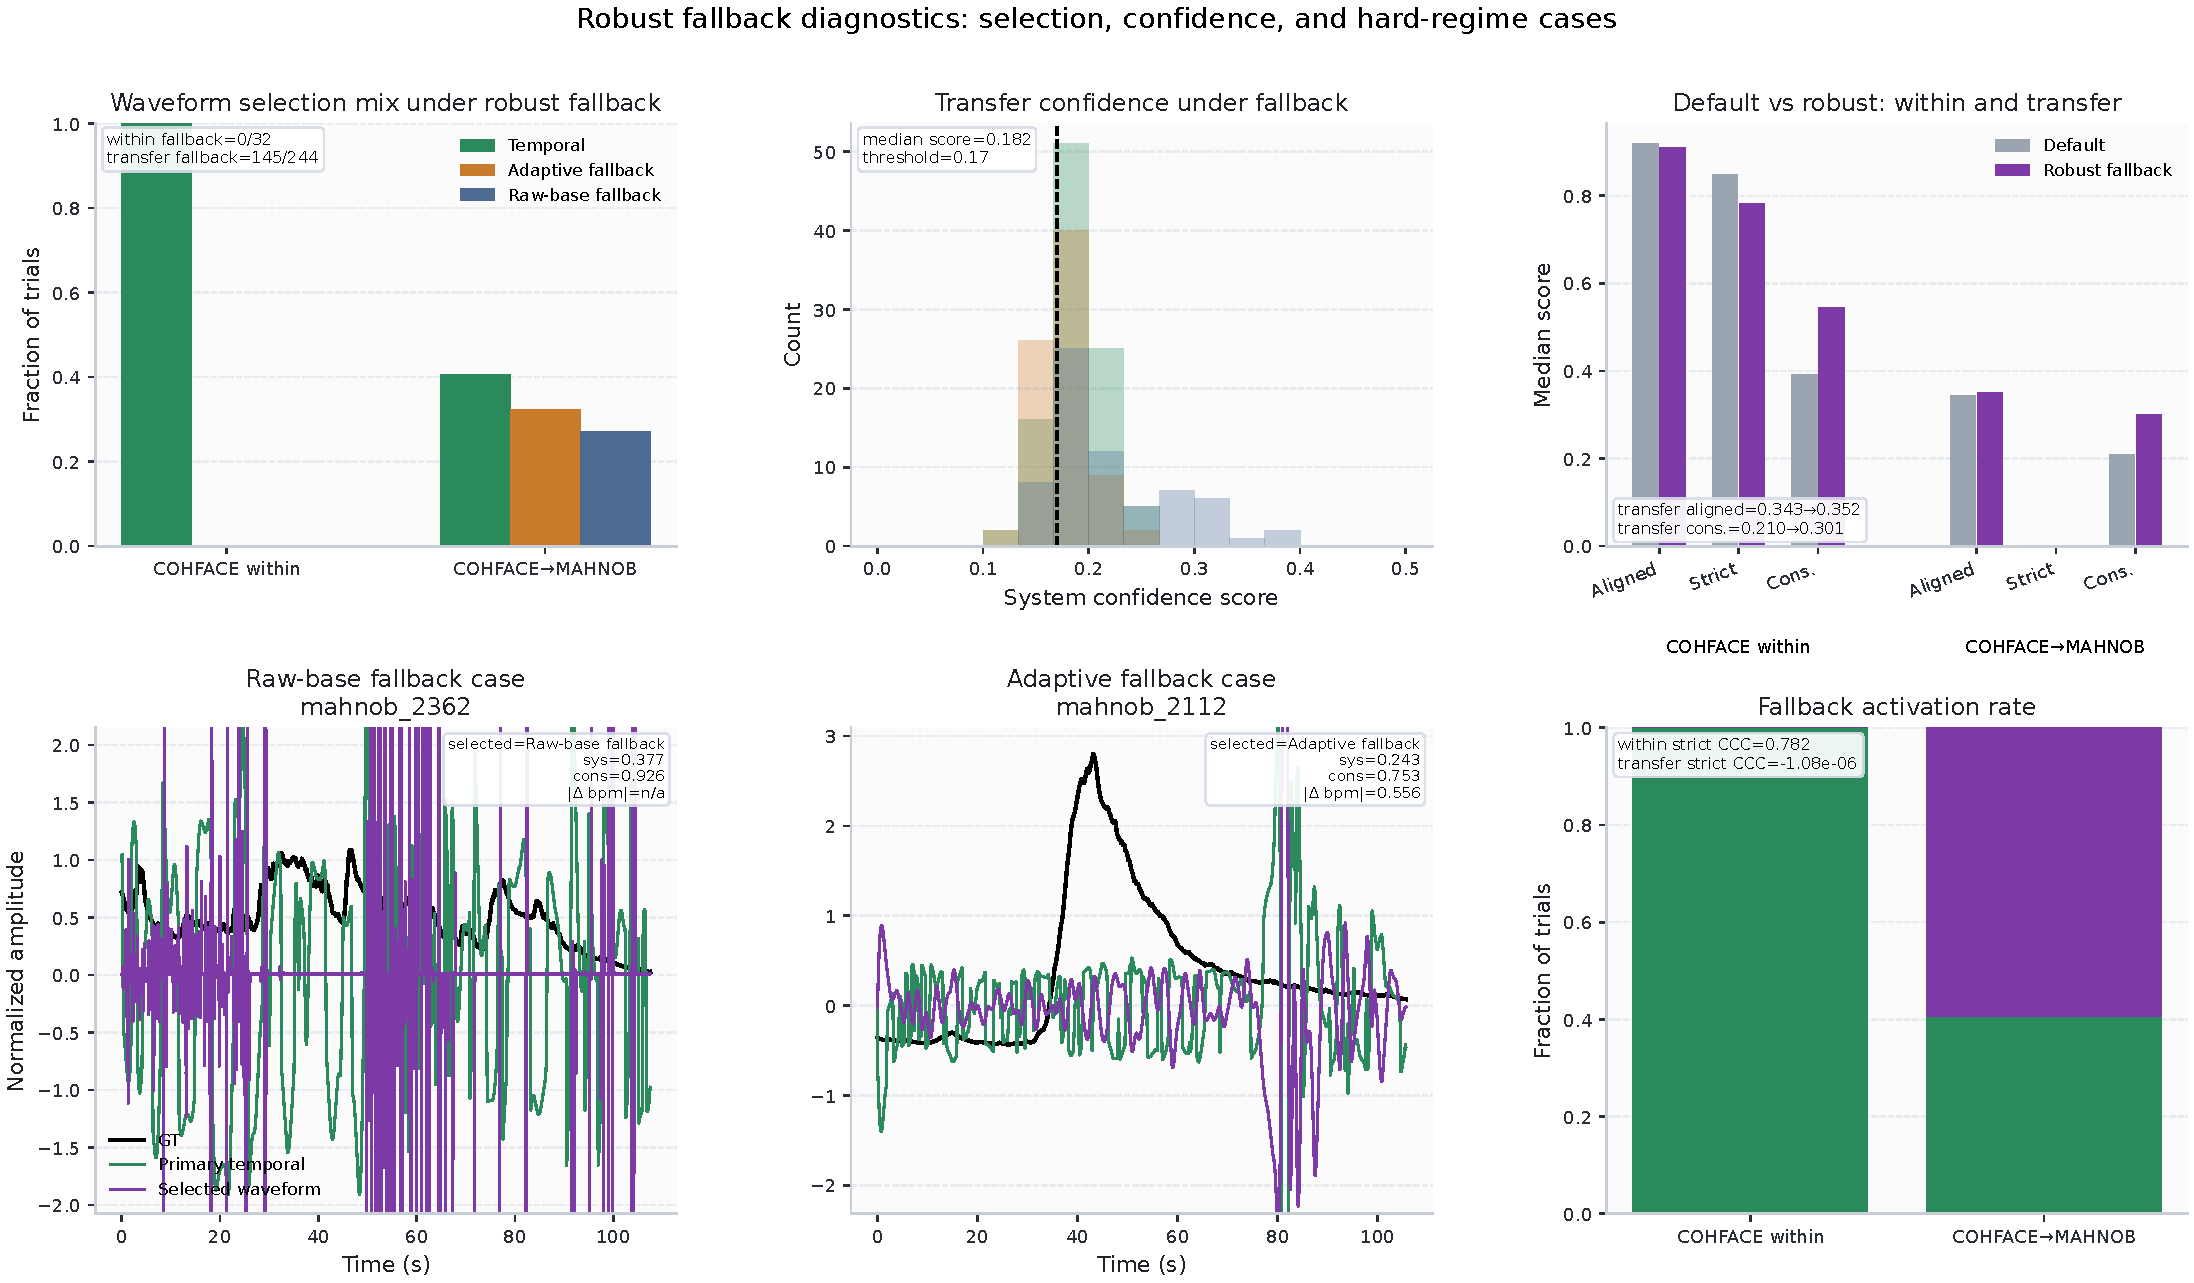
\includegraphics[width=0.90\linewidth]{figures/S_F11_robust_fallback_diagnostics.pdf}
\caption{Robust-fallback diagnostics. The fallback analyses are retained as hard-regime diagnostic evidence and are not promoted as the main operating point.}
\end{figure}

This figure marks the boundary between useful hard-regime diagnostics and the
reported operating point. The fallback behaviour is informative about weak
observability and nuisance pressure, but it is not used to replace the
predefined PARH-OSSM evaluation route.

\begin{figure}[htbp]
\centering
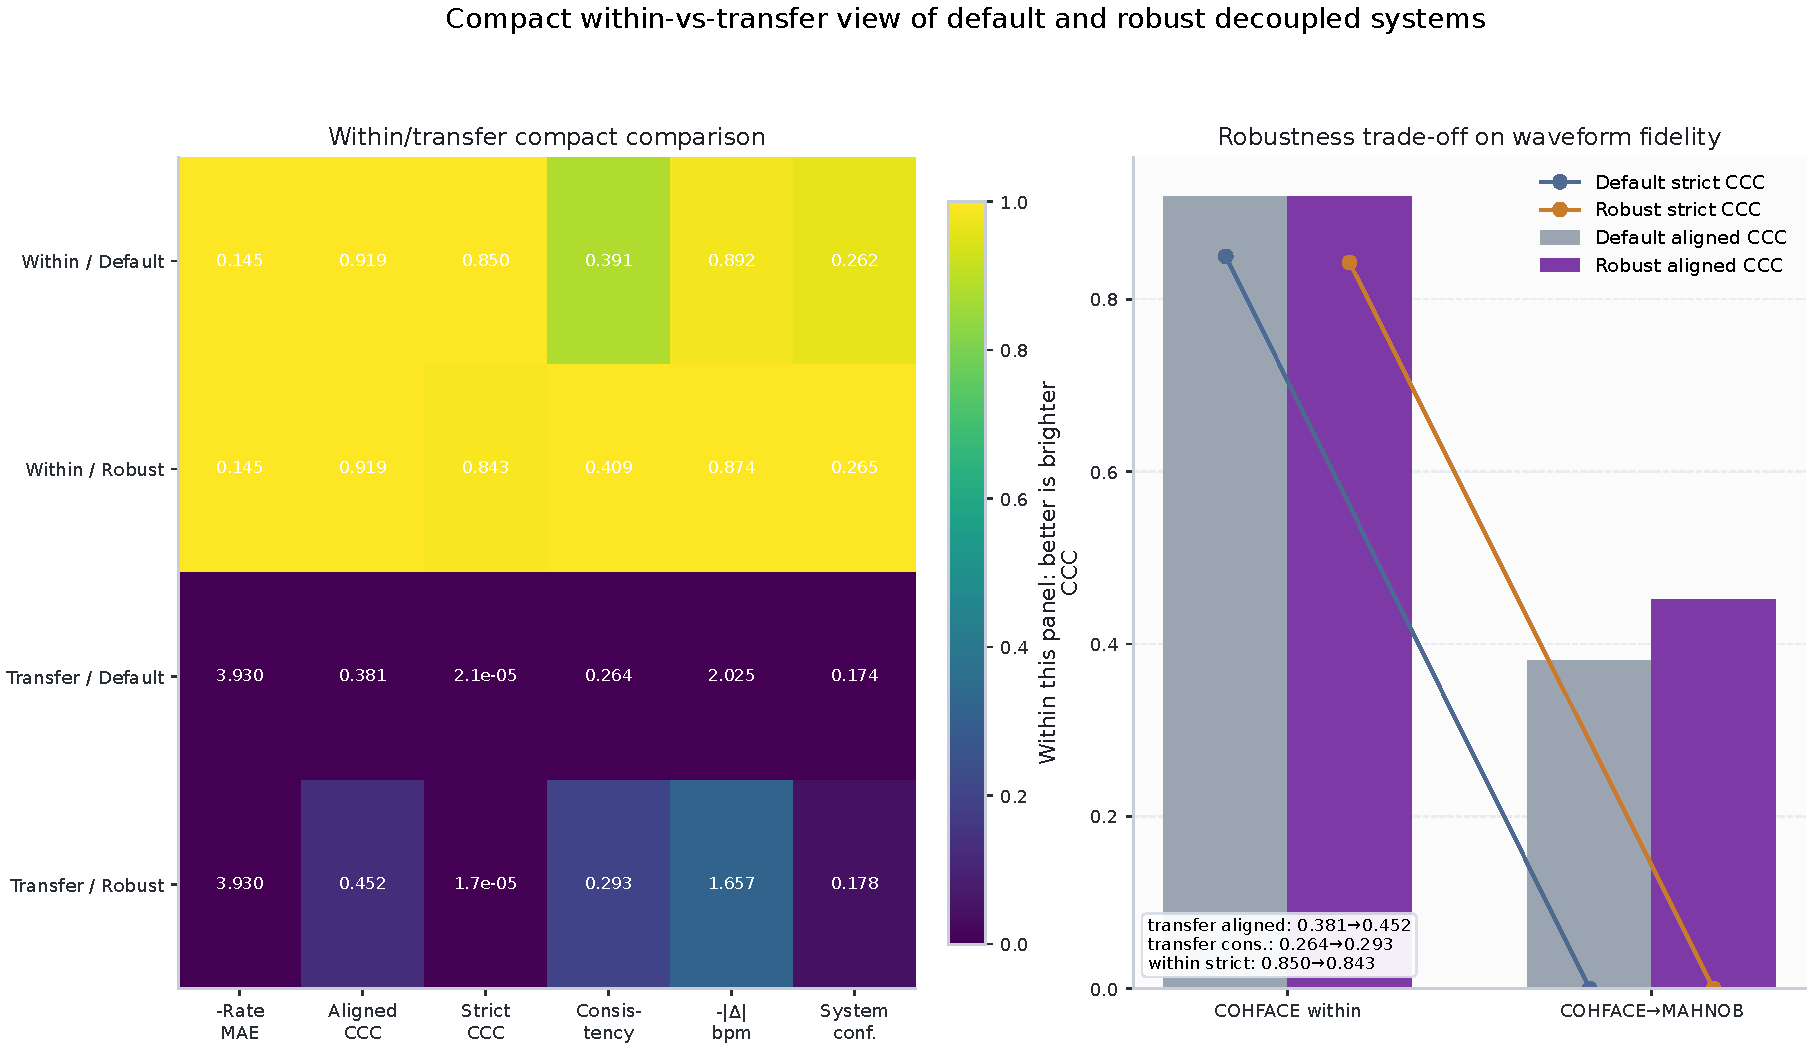
\includegraphics[width=0.90\linewidth]{figures/S_F12_within_transfer_compact_comparison.pdf}
\caption{Within-versus-transfer operating-point comparison. The figure is retained as diagnostic context for readout policy boundaries.}
\end{figure}

This figure checks whether operating-point behaviour is stable within and
across evaluation settings. It is included to document readout-policy
boundaries, not to introduce an additional tuned model variant.

\begin{figure}[htbp]
\centering
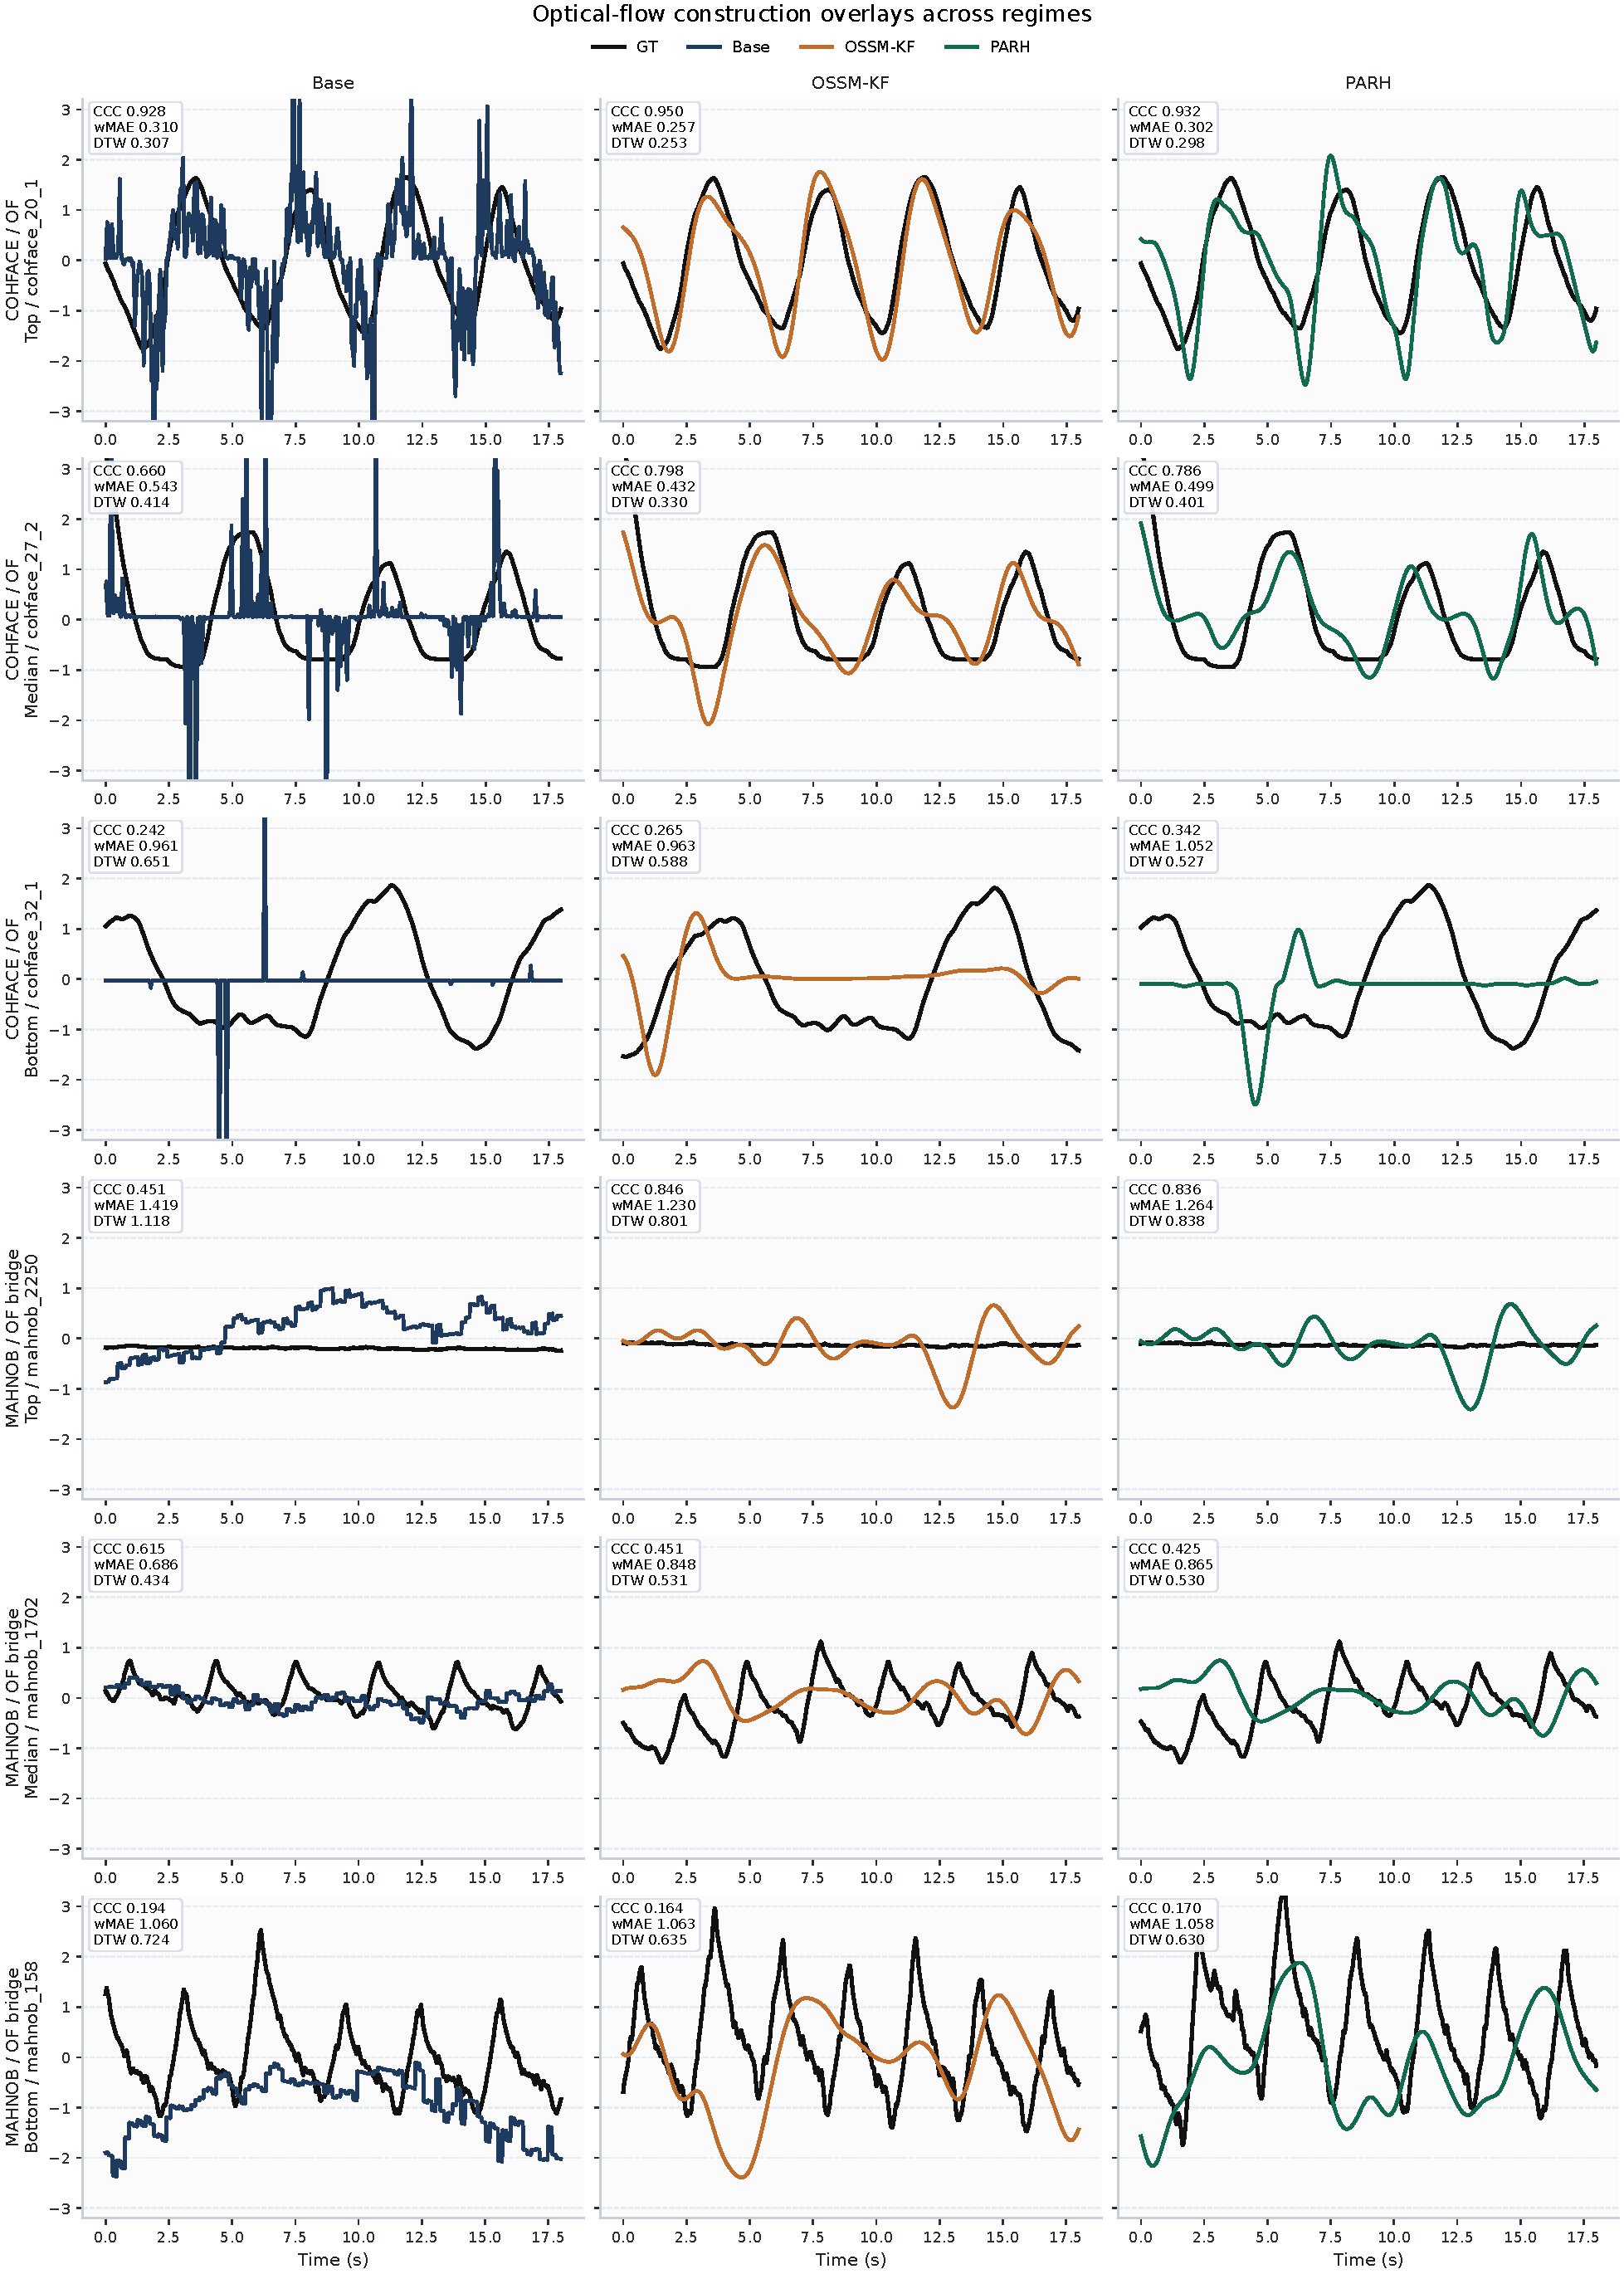
\includegraphics[width=\linewidth,height=0.78\textheight,keepaspectratio]{figures/S_F13_of_construction_overlay_grid.pdf}
\caption{Optical-flow construction overlay companion. The panels show OF and OF-bridge behavior under the same visual grammar as the main overlay atlas.}
\end{figure}

This overlay companion makes the OF construction claim visually auditable. The
same reference grammar is used for raw OF and OF-bridge, so differences between
the panels reflect observation construction rather than a change in plotting or
case-selection logic.

\begin{figure}[htbp]
\centering
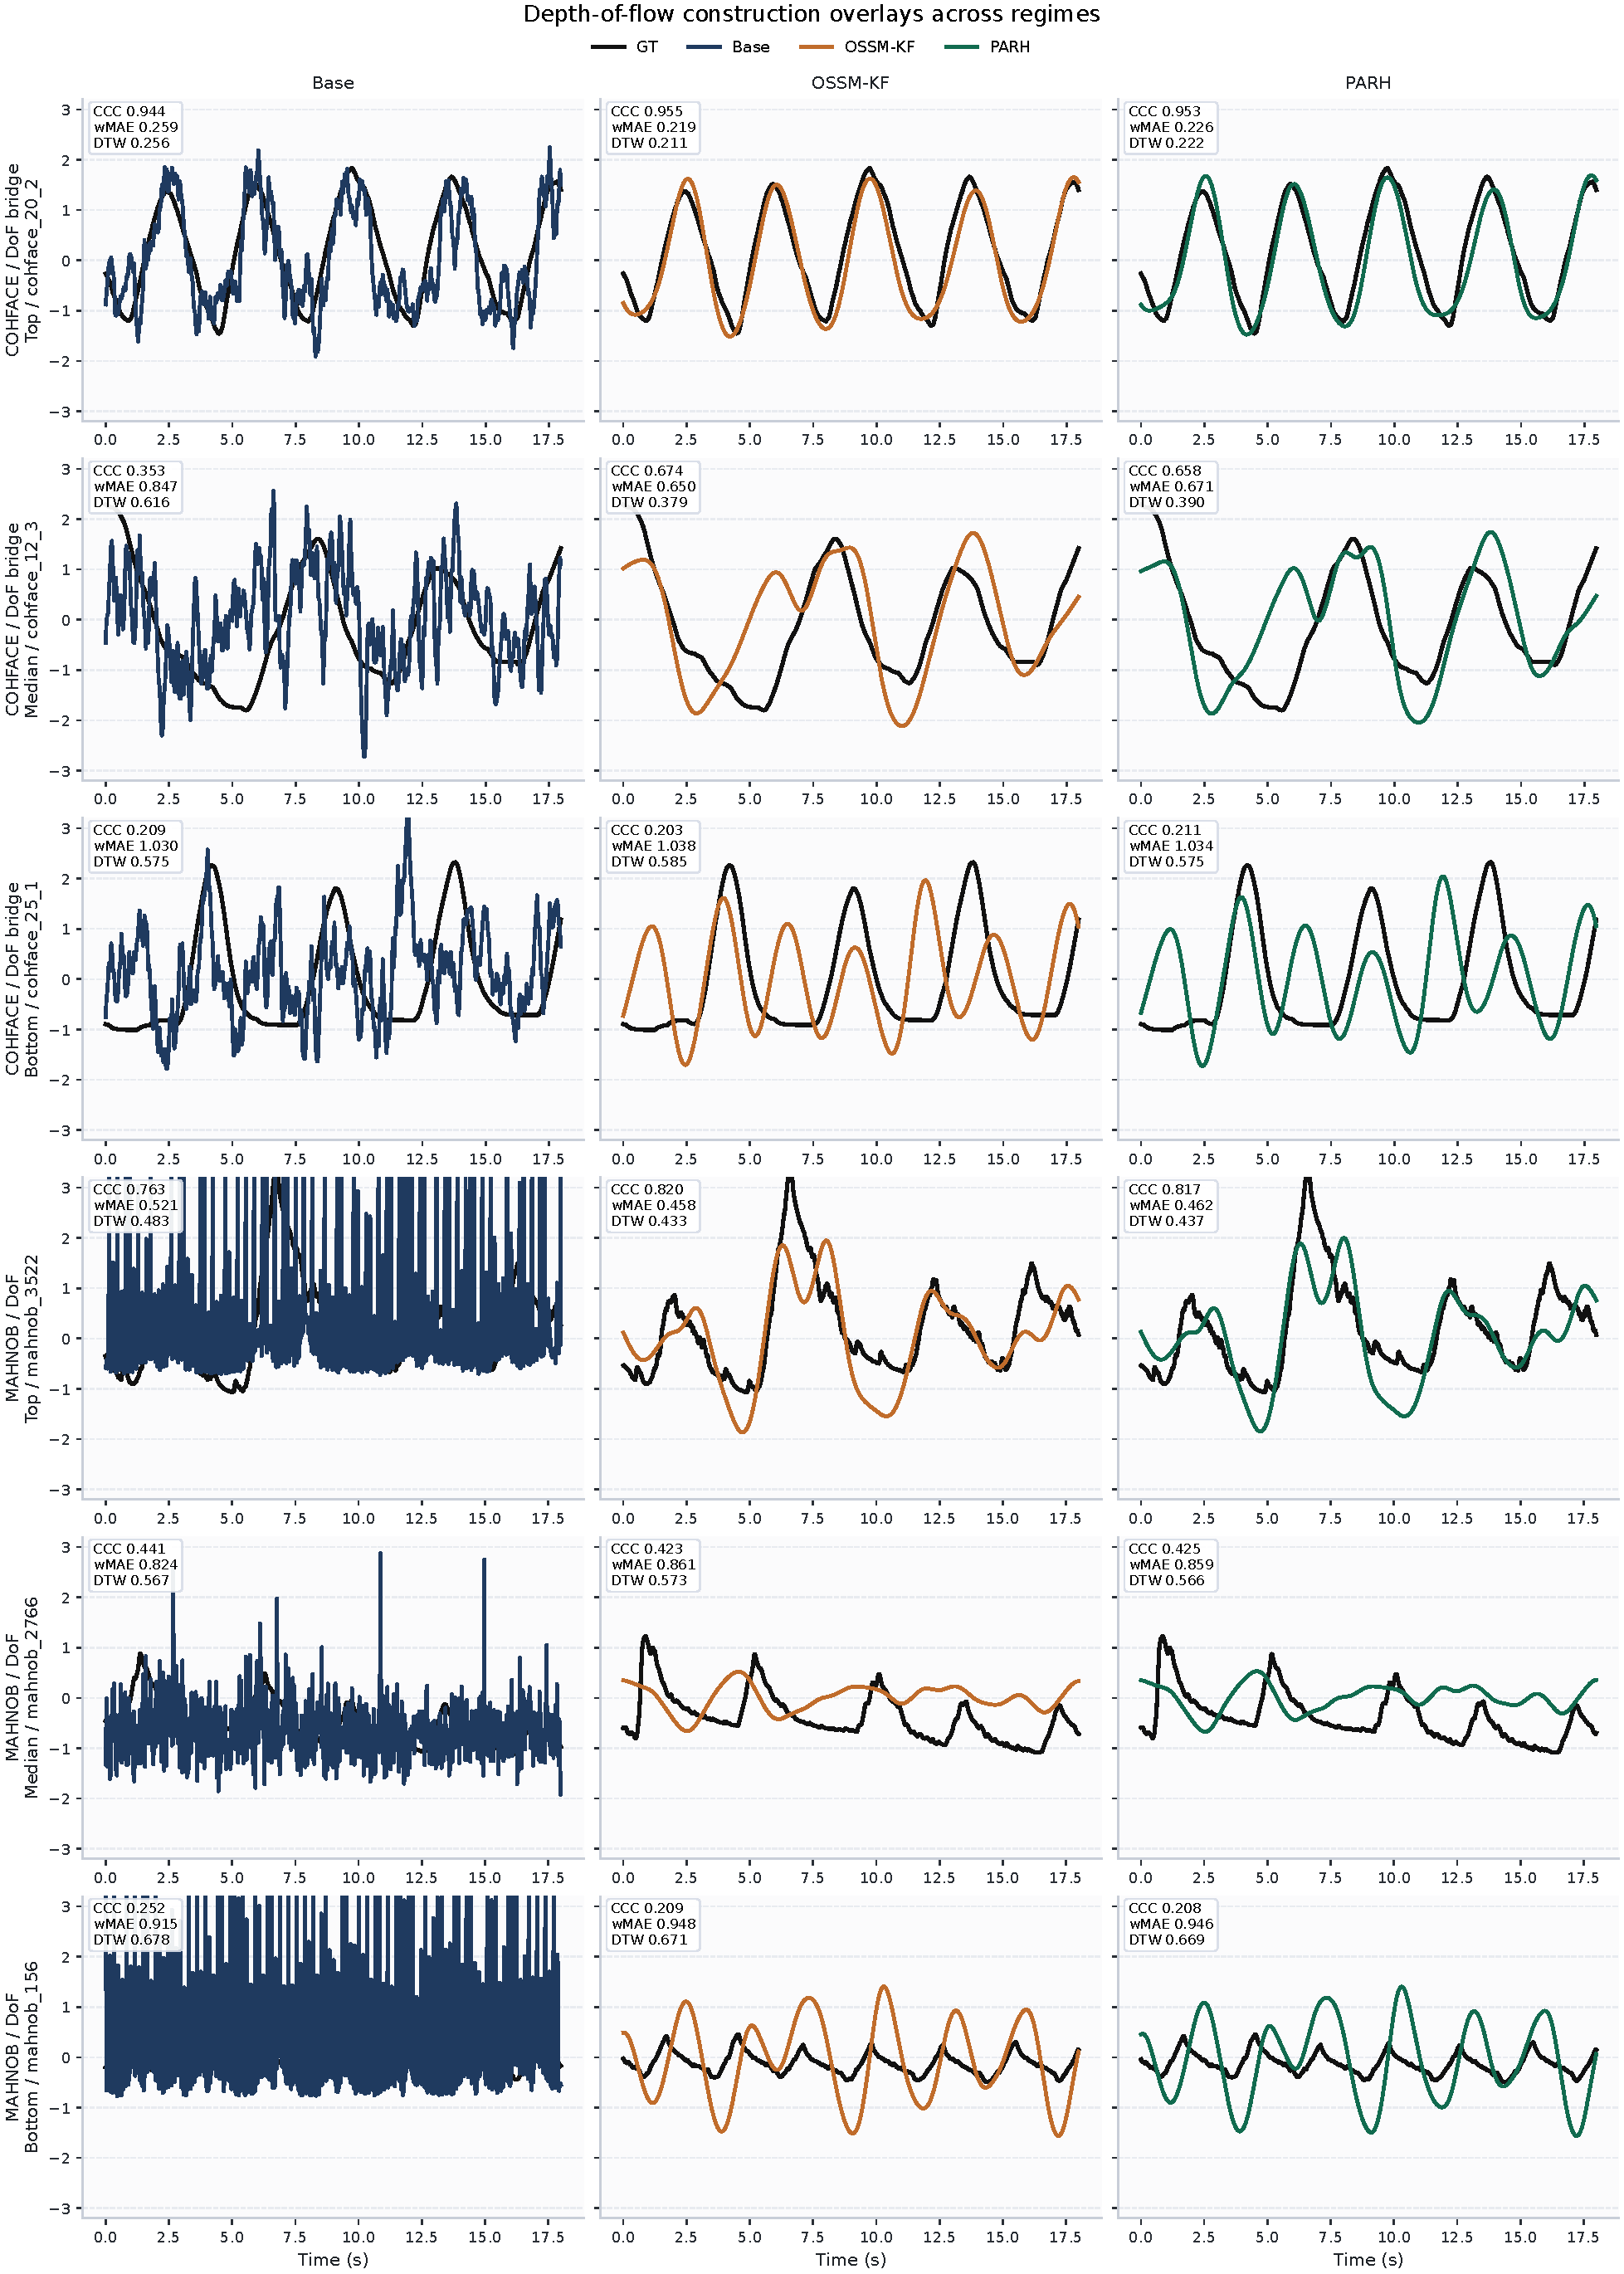
\includegraphics[width=\linewidth,height=0.78\textheight,keepaspectratio]{figures/S_F14_dof_construction_overlay_grid.pdf}
\caption{Depth-of-flow construction overlay companion. The panels show DoF and DoF-bridge behavior as construction-level diagnostic context.}
\end{figure}

This overlay companion performs the same construction-level check for DoF and
DoF-bridge. It helps identify whether thresholded motion energy and signed
centroid motion expose the same respiratory structure or fail through different
nuisance mechanisms.

\begin{figure}[htbp]
\centering
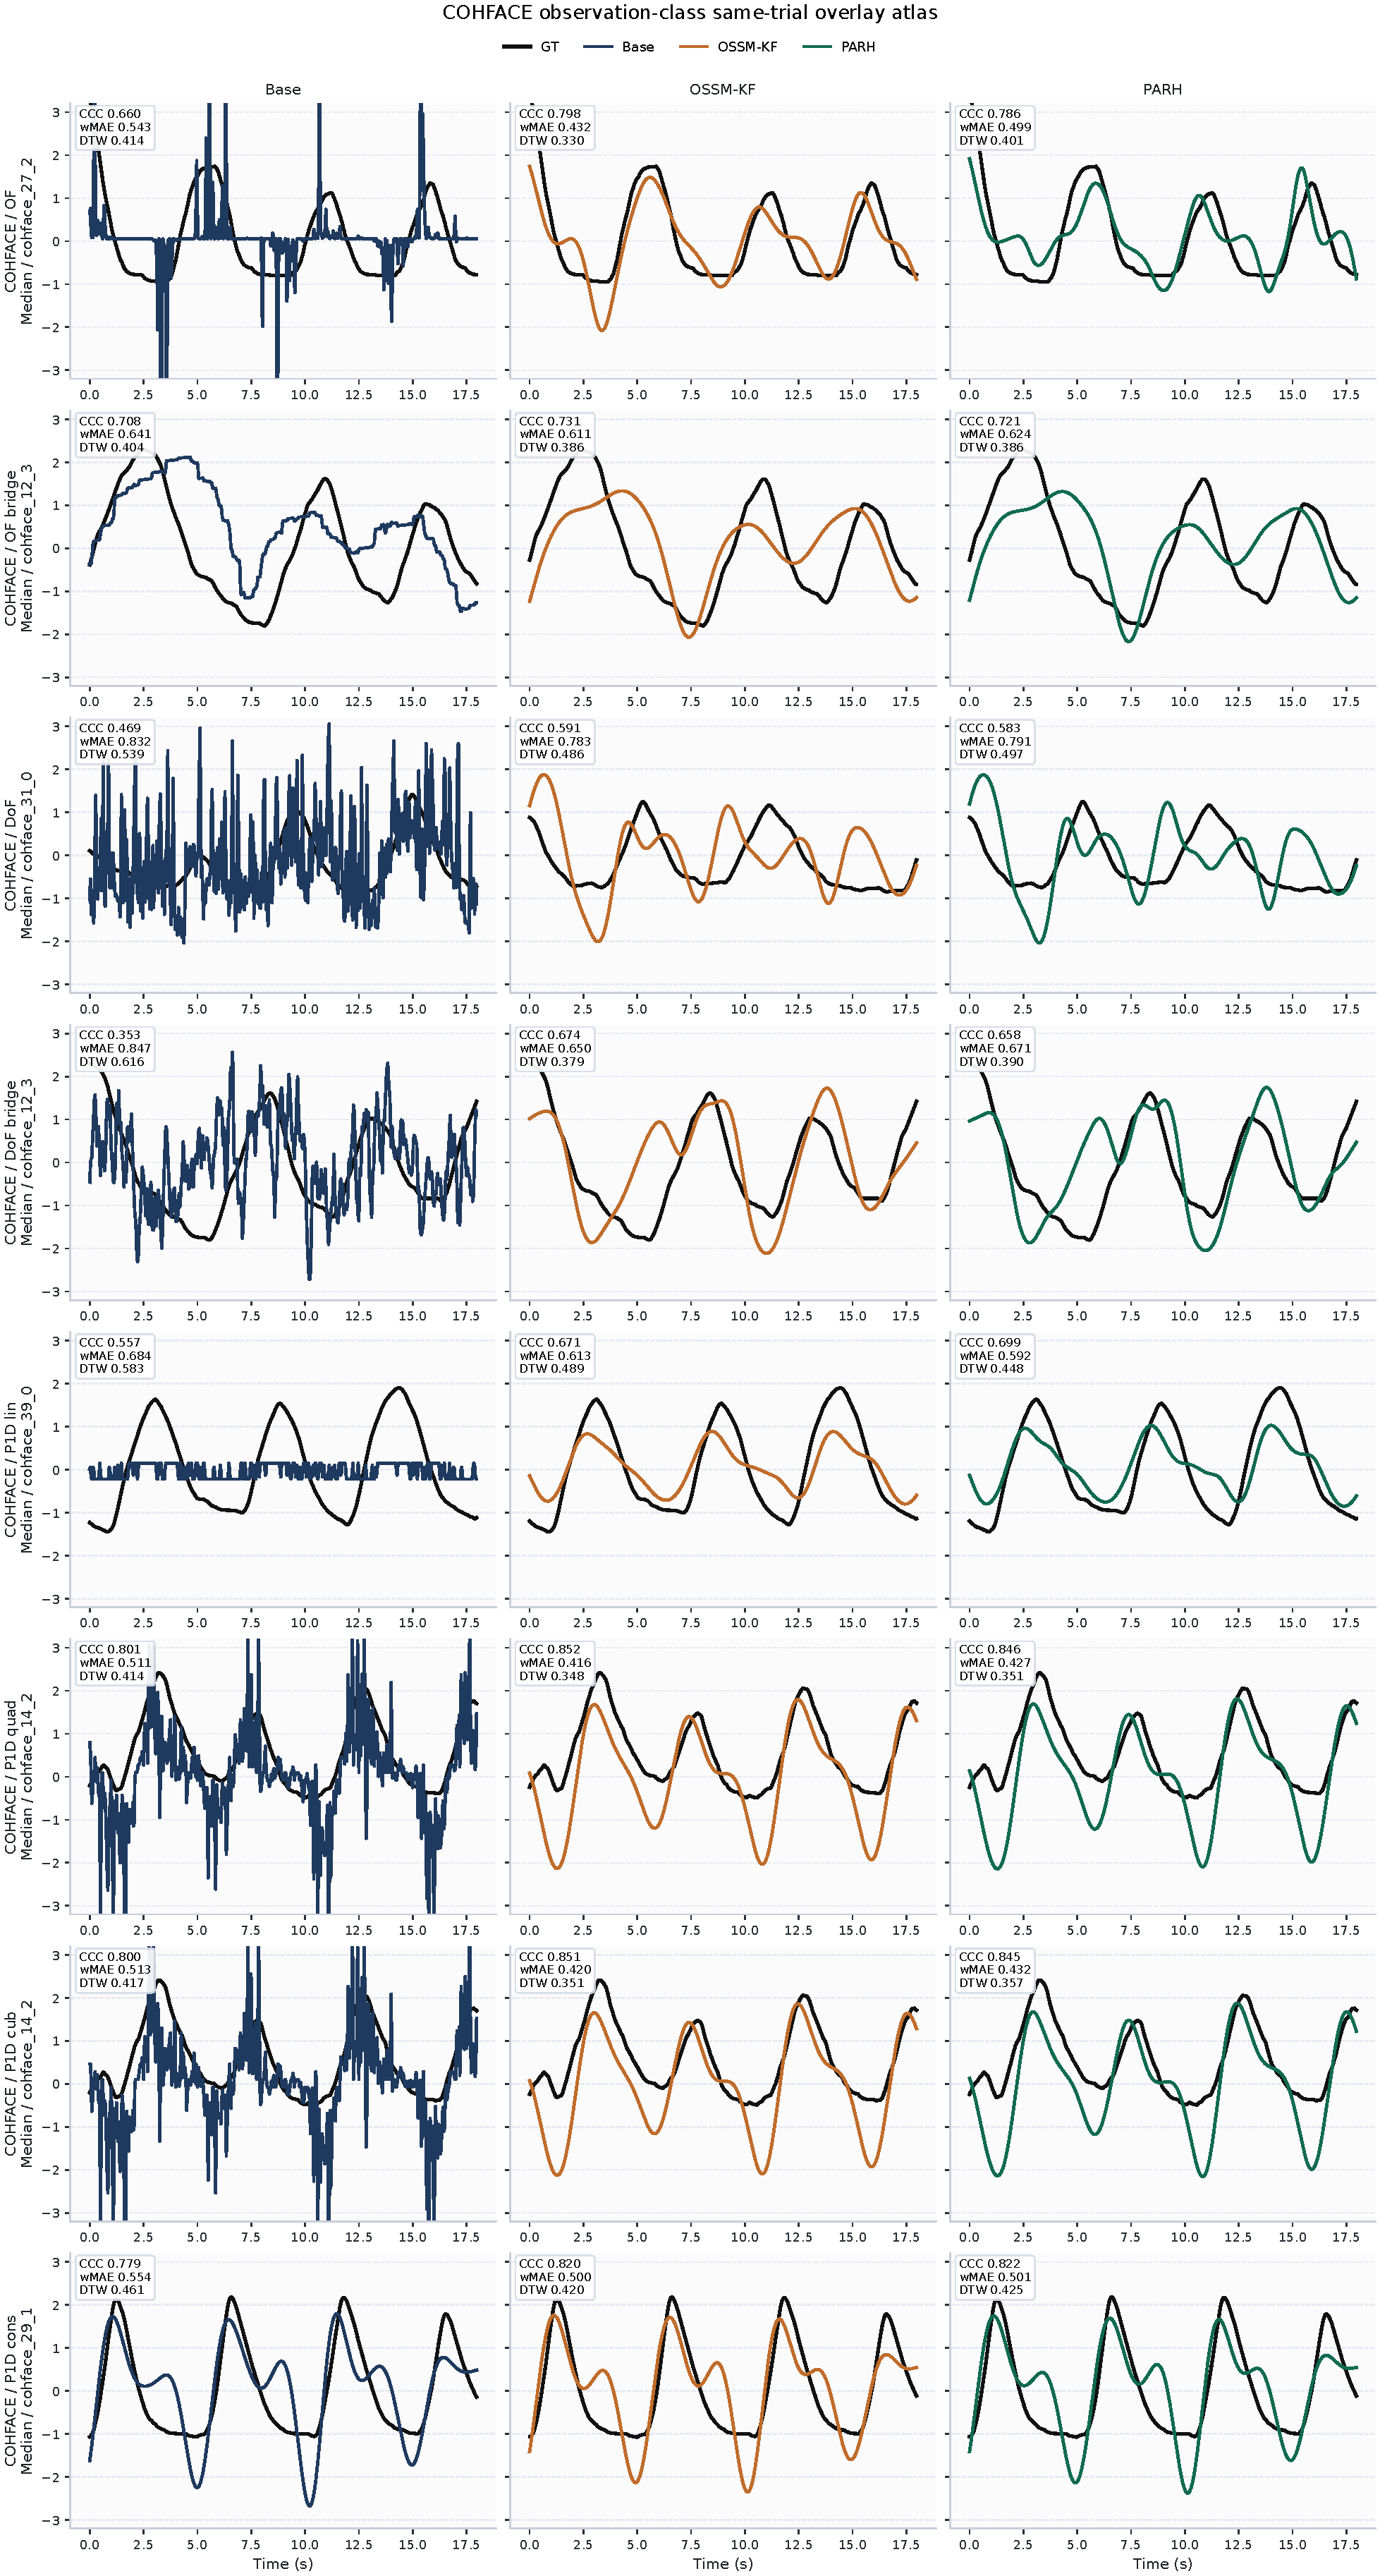
\includegraphics[width=\linewidth,height=0.78\textheight,keepaspectratio]{figures/S_F15_cohface_observation_class_overlay_atlas.pdf}
\caption{COHFACE observation-median all-class overlay atlas. The figure expands the clean-regime waveform topology evidence beyond the single main-text case.}
\end{figure}

This atlas shows whether the clean-regime visual pattern in the main text is
representative across observation classes. It supports the interpretation that
COHFACE contains strong native respiratory evidence in several fixed
observation routes.

\begin{figure}[htbp]
\centering
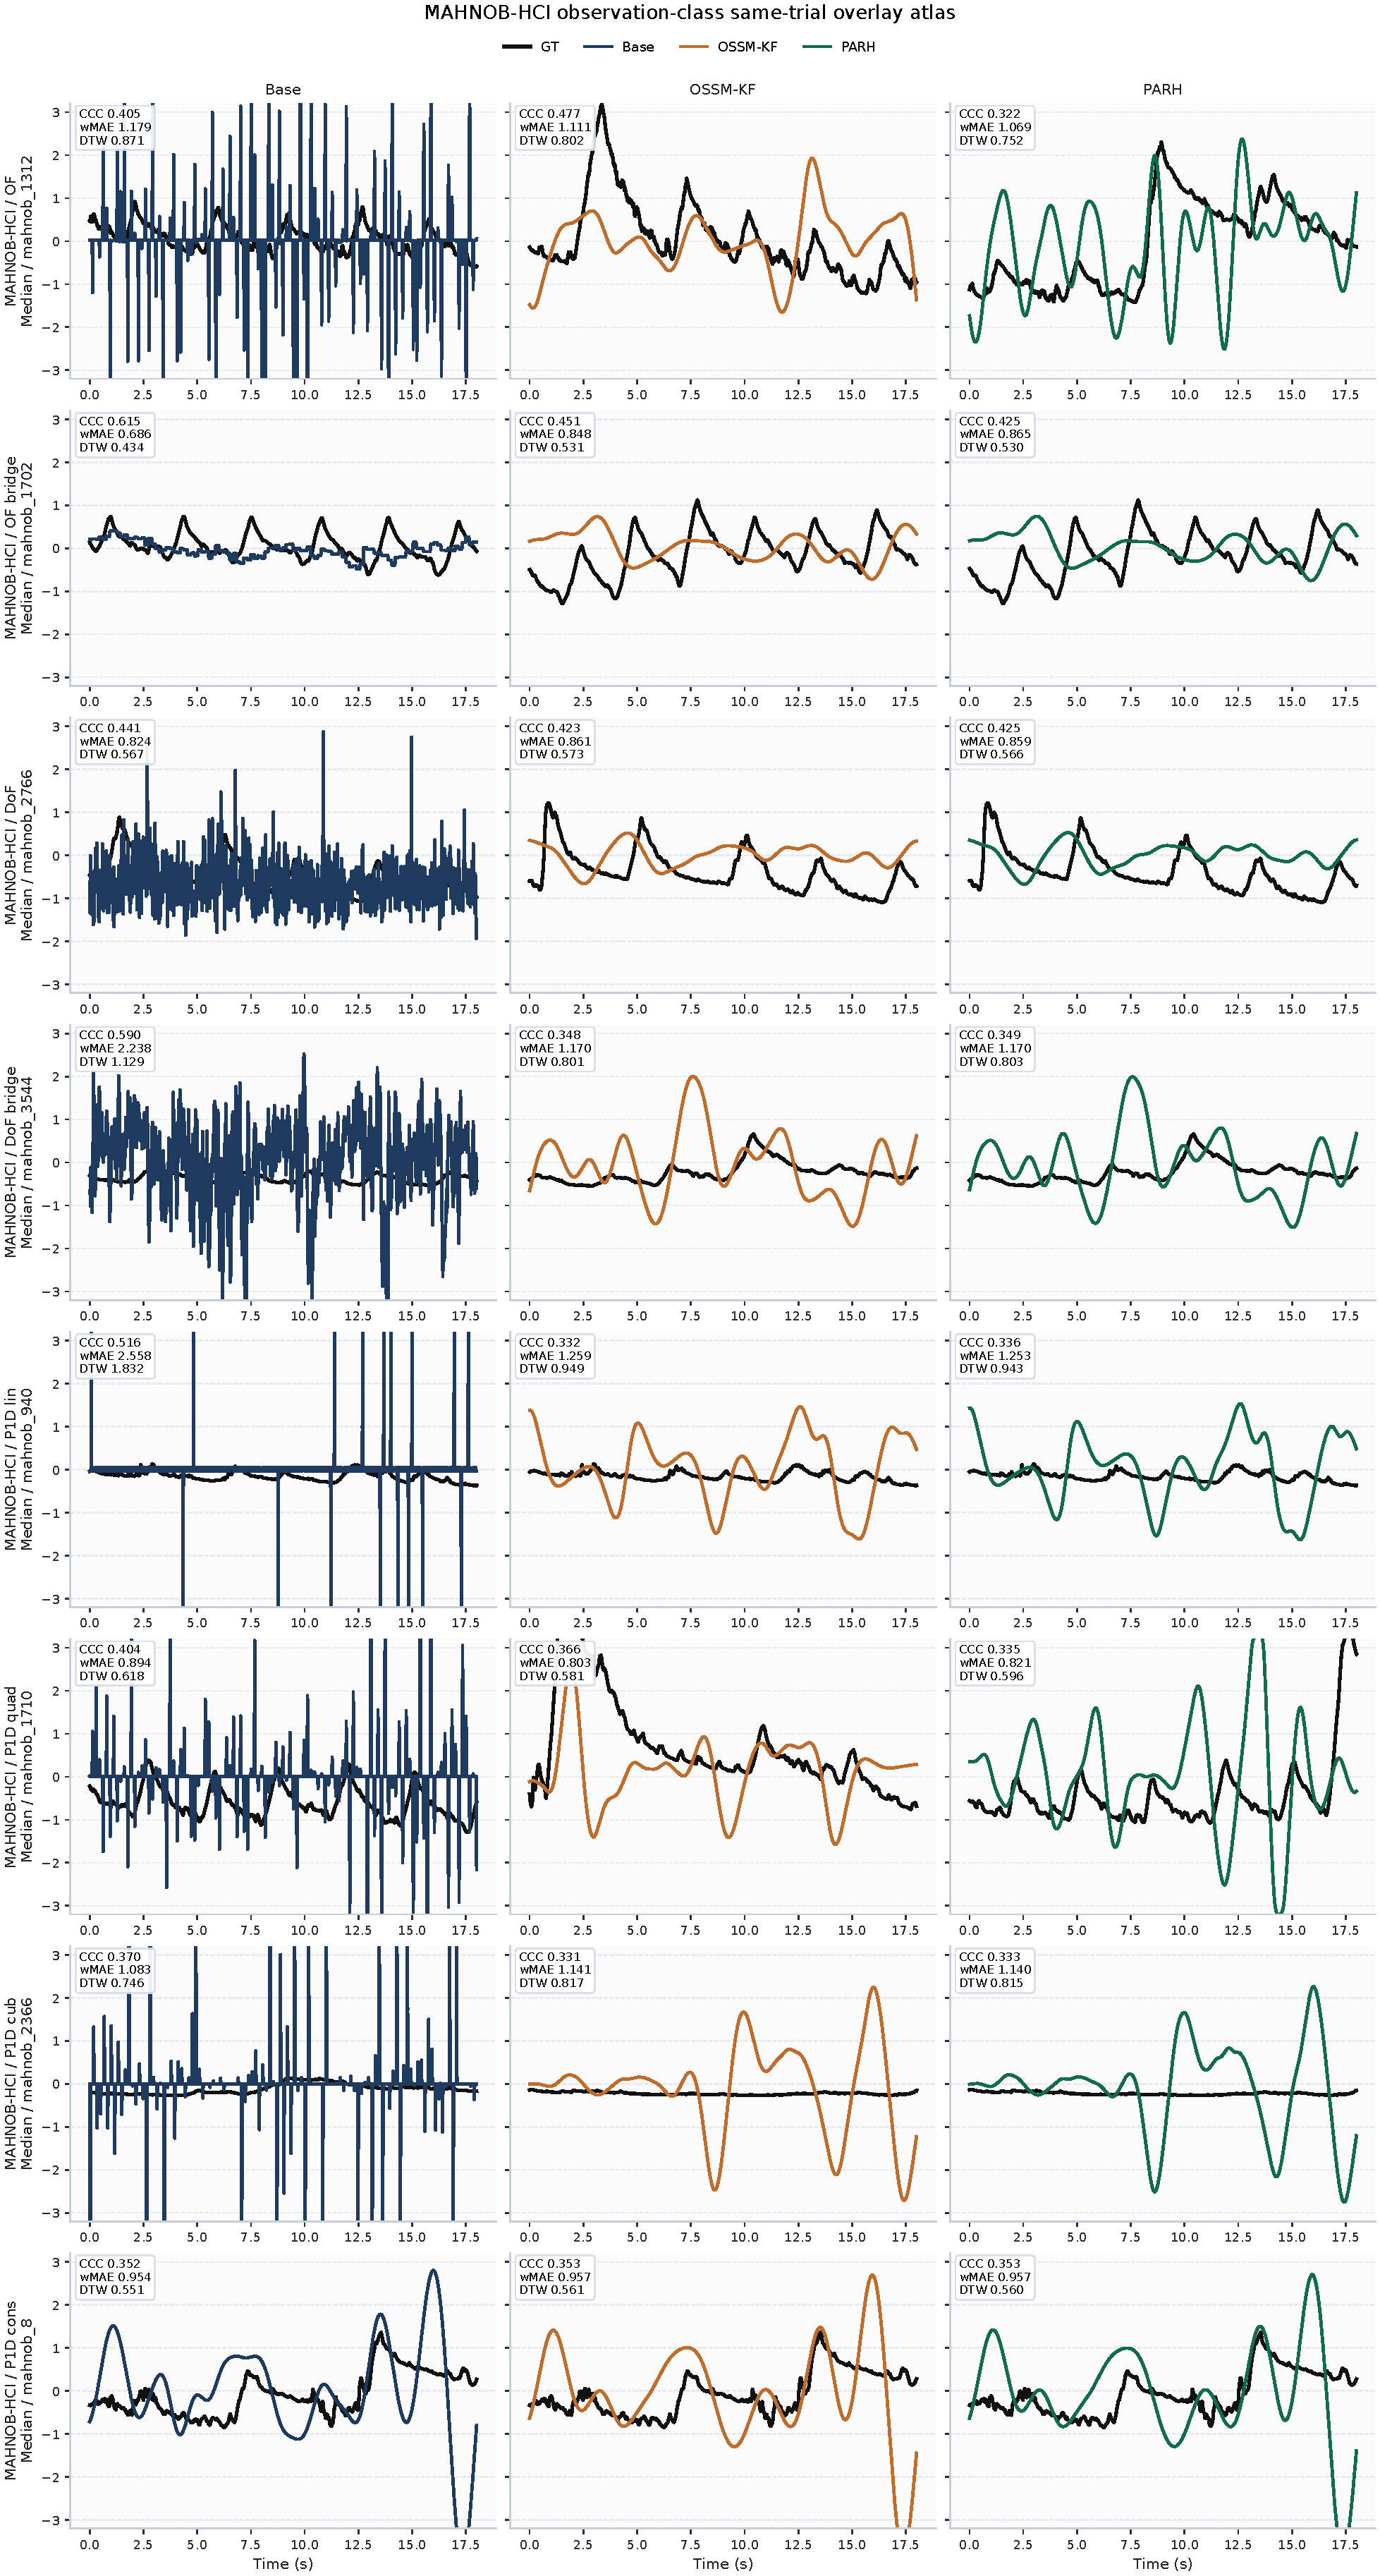
\includegraphics[width=\linewidth,height=0.78\textheight,keepaspectratio]{figures/S_F16_mahnob_observation_class_overlay_atlas.pdf}
\caption{MAHNOB-HCI observation-median all-class overlay atlas. The figure expands the hard-regime waveform topology evidence and helps localize low-observability behavior.}
\end{figure}

This atlas is the hard-regime counterpart to the COHFACE overlay companion. It
shows that MAHNOB-HCI failures are not only final-readout errors; weak or
inconsistent observation topology is already visible across the fixed
observation bank.

\end{document}
